% -*- program: xelatex -*-
\documentclass[11pt, compress]{beamer} 

%\usefonttheme[onlymath]{serif}
\DeclareFontEncoding{T1}
\fontencoding{T1}
\usepackage[T2A]{fontenc}
\usepackage[utf8]{inputenc}
\usepackage[russian]{babel}
\usepackage{listings}
\usepackage{amsmath,amssymb,amsthm,mathabx}
\hypersetup{unicode=true}
\usepackage{color}
\definecolor{mygreen}{RGB}{28,172,0} % color values Red, Green, Blue
\definecolor{mylilas}{RGB}{170,55,241}
\definecolor{codecolor}{RGB}{0,120,0}
\newcommand{\matcode}[1]{ \textcolor{codecolor}{\texttt{#1}}}
\usepackage{graphics,graphicx}
\usepackage{verbatim}
\usepackage{fancyvrb}
\usepackage{booktabs}
%\usepackage{media9}

 
\newcommand{\cleartitlepage}[1]{\begin{frame}[plain]\begin{center}\textsc{#1}\end{center}\end{frame}}
\usetheme{m} 

\usepackage{tikz}
\usetikzlibrary{positioning} 
\tikzset{cbutton/.style={rectangle,minimum width=10mm,thick,draw=red!50!black!50,
top color=white,bottom color=red!50!black!30}}
\tikzset{mbutton/.style={rectangle,minimum width=10mm,thick,draw=black!20,
top color=white,bottom color=black!30}}

\lstset{language=Matlab,    
    keepspaces=true,
    extendedchars=true,
    basicstyle={\footnotesize  \color{black}},
    breaklines=true,
    morekeywords={matlab2tikz},
    keywordstyle=\color{blue},
    morekeywords=[2]{1}, keywordstyle=[2]{\color{codecolor}},
    identifierstyle={ \bf \color{black} },
    stringstyle=\color{mylilas},
    commentstyle=\color{mygreen},%
    showstringspaces=false,
    numbers=left,%
    numberstyle={\tiny \color{black}},
    numbersep=7pt, 
    emph=[1]{case,switch,otherwise},emphstyle=[1]\color{blue}, 
    frame=single,    
    %lineskip=-1.0pt,
    %emph=[2]{word1,word2}, emphstyle=[2]{style},    
}

\title{Орбитальное движение}
\subtitle{Компьютерный практикум по механике}
\author{Юдинцев В. В.}
\small
\institute[СГАУ]
{
Кафедра теоретической механики \\
Самарский государственный аэрокосмический университет \\ им. академика С.~П.~Королёва \\
(национальный исследовательский университет) \\
\vfill
{http://yudintsev.info}
}

\begin{document}

{
\usebackgroundtemplate{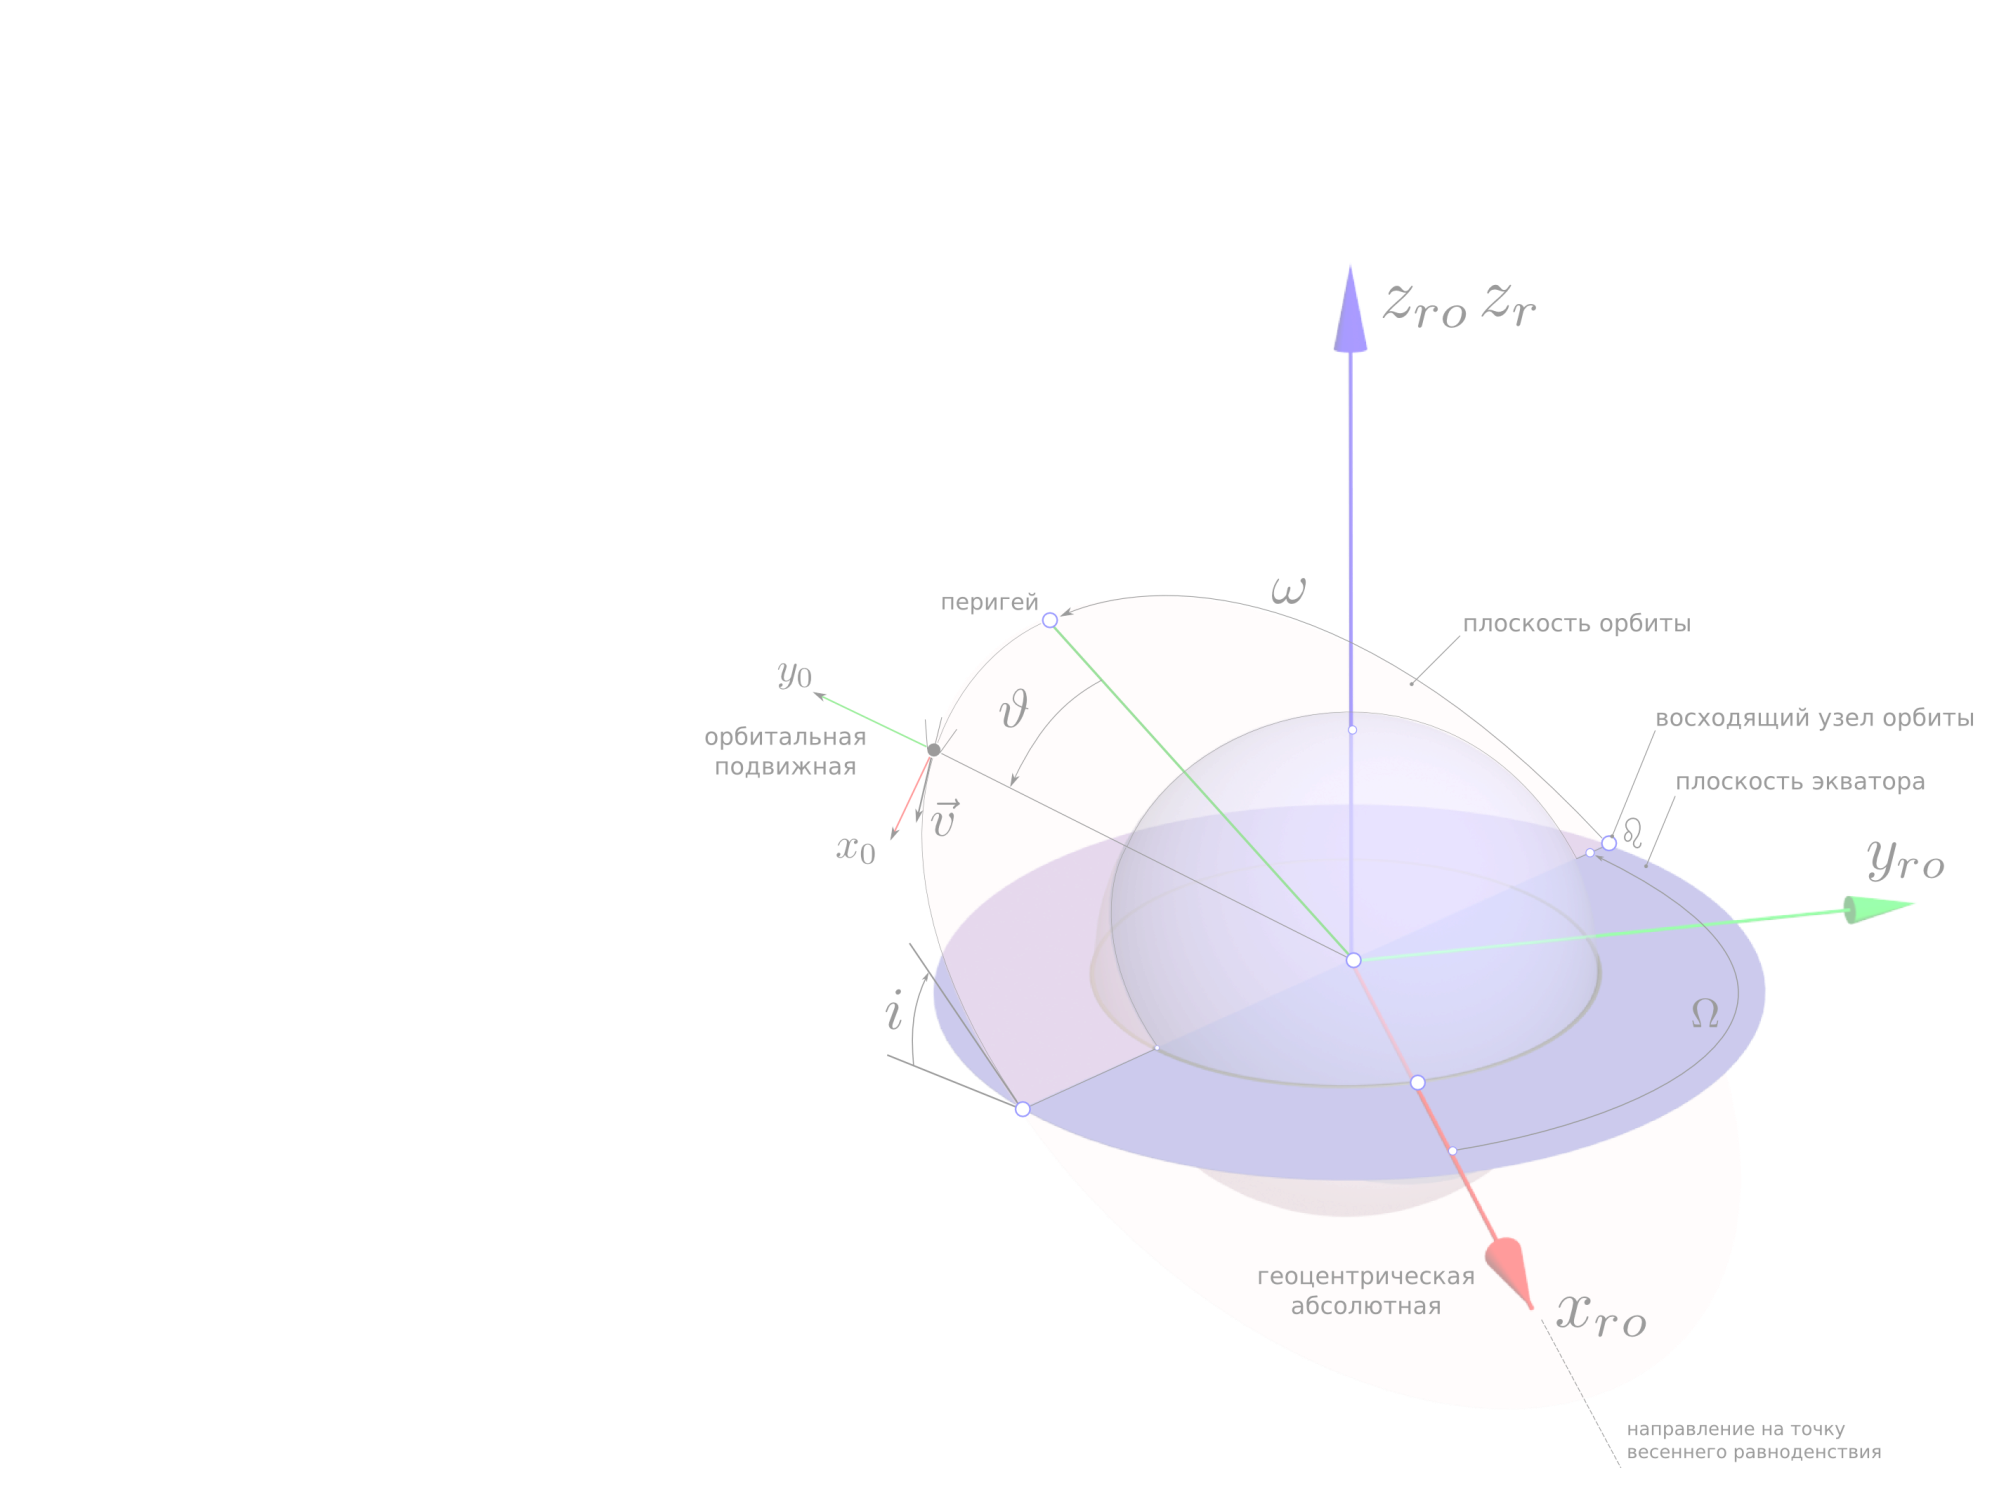
\includegraphics[width=\paperwidth,height=\paperheight]{./Orbital.png}}
\maketitle
} 

\frame{
\frametitle{Содержание}
\tableofcontents
}
%
%
\section{Движение материальной точки в центральном поле}
%
%
\begin{frame}[fragile]{Геоцентрическая инерциальная система координат $OXYZ$}
\begin{figure}[htbp]
  \centering
  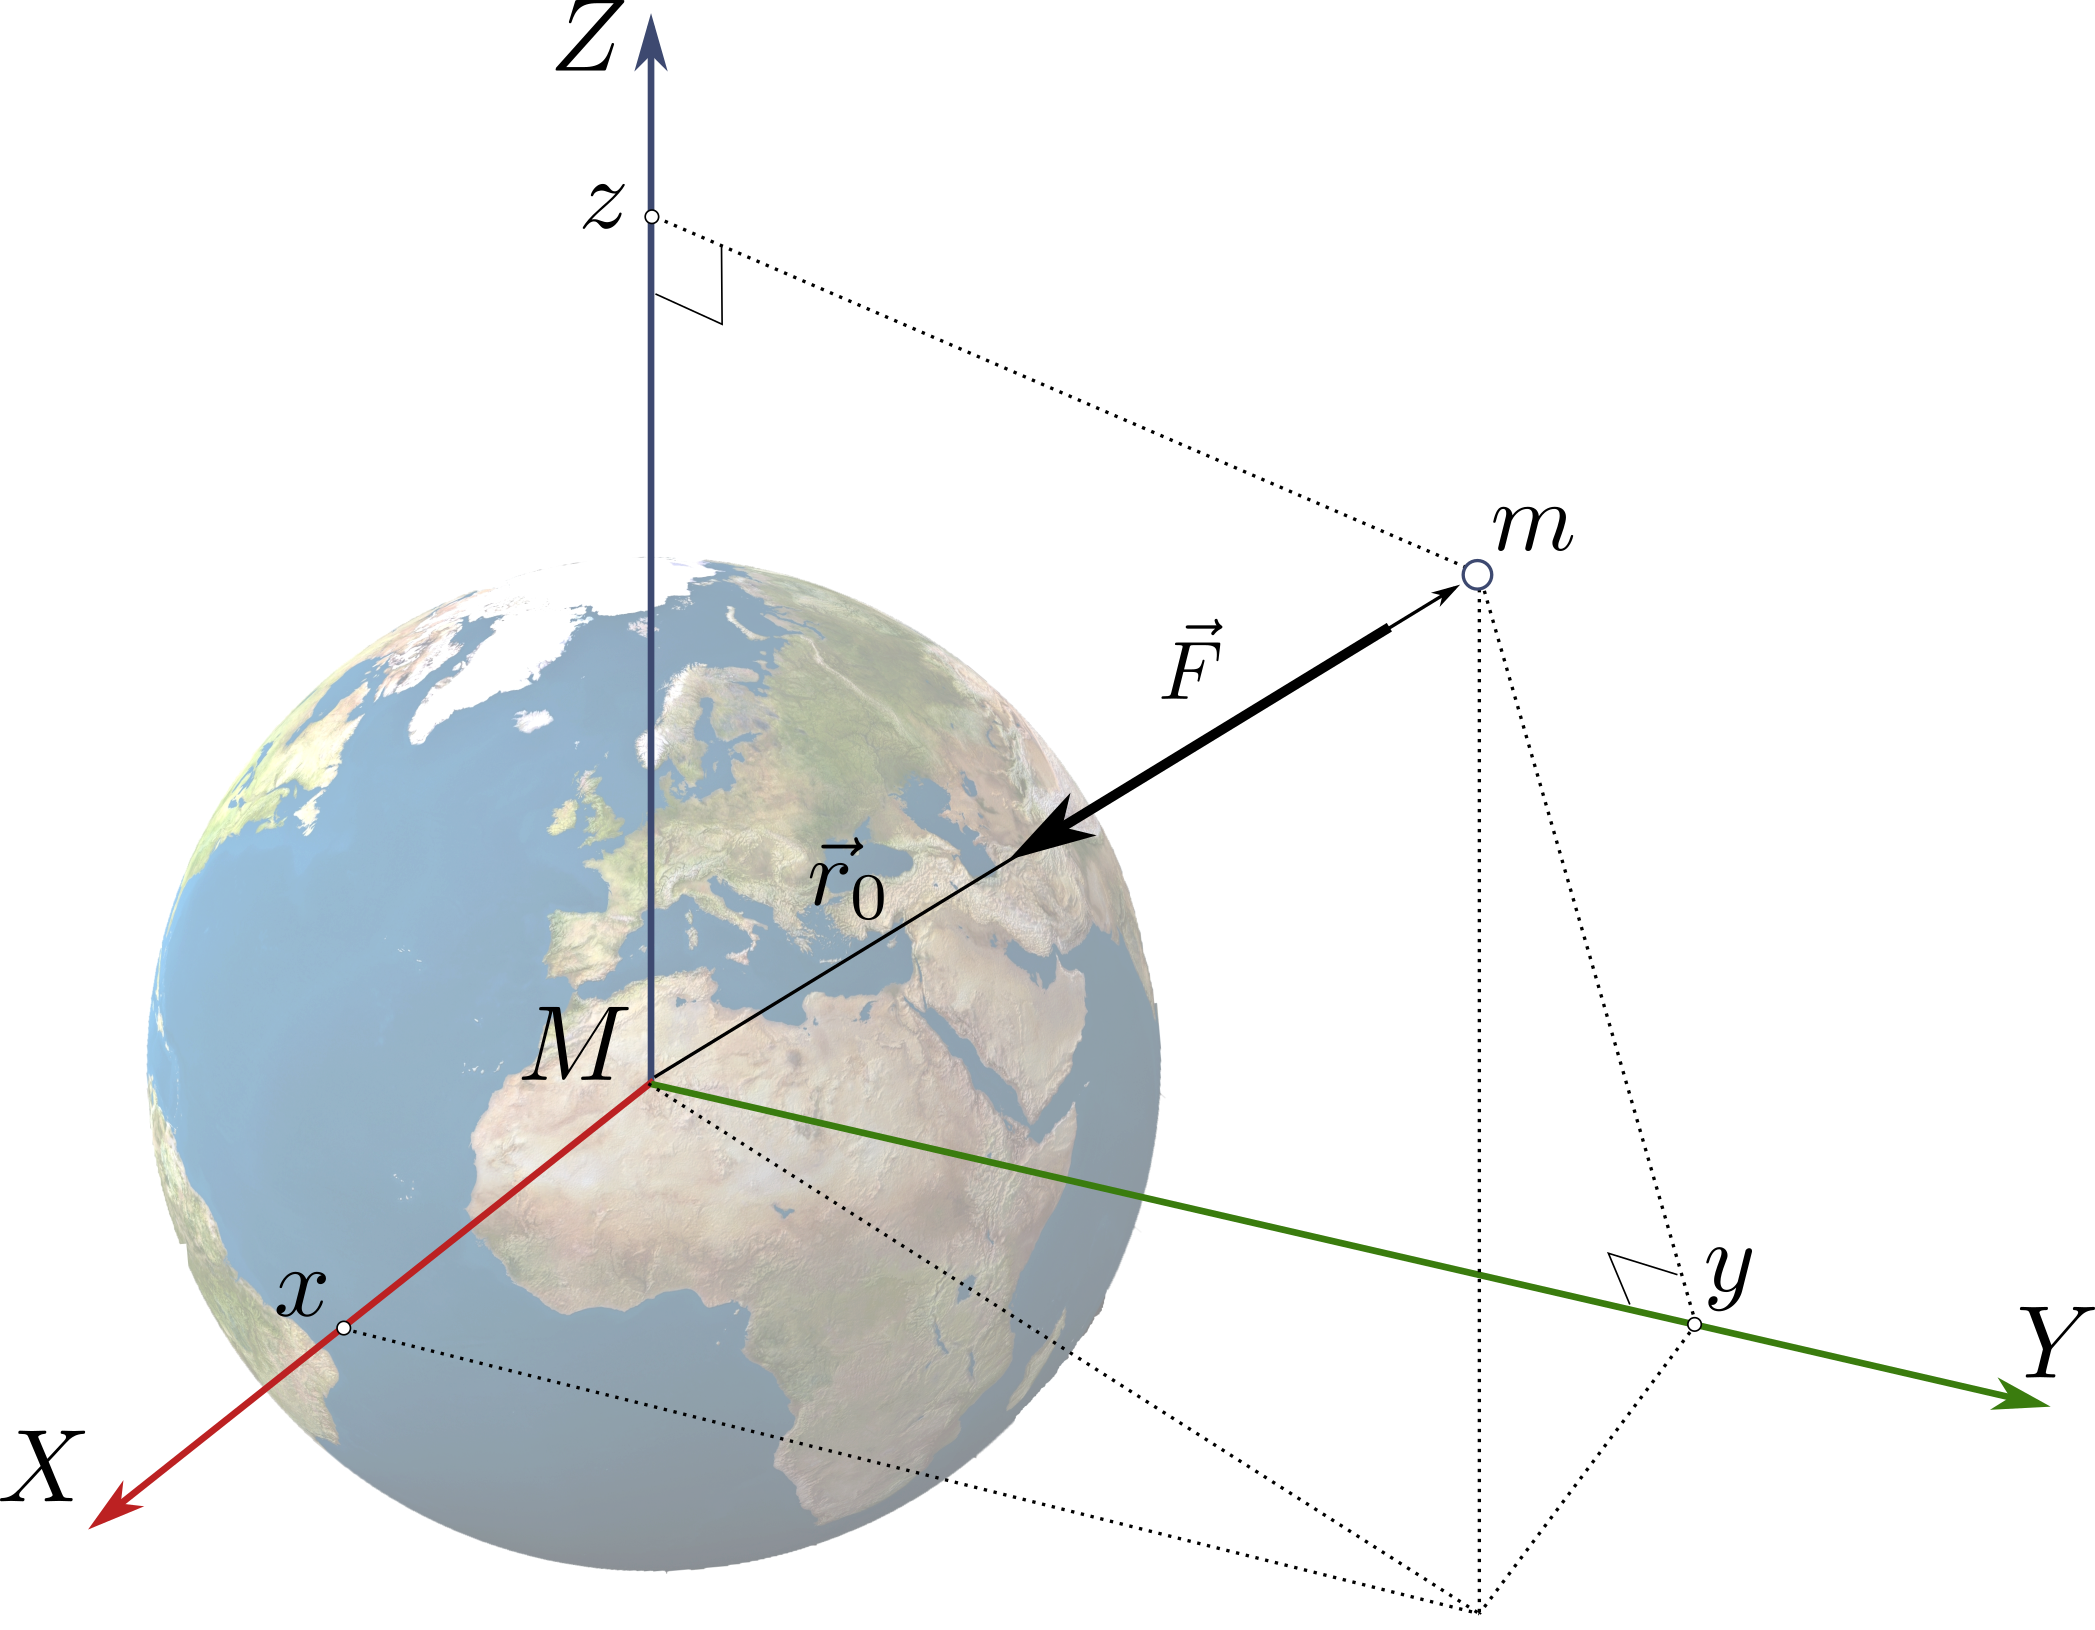
\includegraphics[width=0.8\textwidth]{ECI.png}  
\end{figure}
\end{frame}


\begin{frame}[fragile]{Движение материальной точки в центральном поле}
Векторная запись:
$$
  m \vec a = \vec F
$$
Модуль силы притяжения Земли, действующей на спутник:
$$
  |\vec F| = F = G \frac{M m}{r_0^2} = \mu \frac{m}{r_0^2}, 
$$ 
где $\mu = G M \approx 3.986\cdot 10^{14}$ м$^3/c^2$ -- гравитационный параметр Земли
\end{frame}


\begin{frame}[fragile]{Уравнения движения}
Векторная запись:
$$
  m \vec a = \vec F
$$
Координатная запись уравнений движения:
$$
\begin{aligned}
  & m a_x = F_x = - F \cos (\widehat{X,-\vec F}) = - F \cos (\widehat{X, r_0}) = - F \cdot{\;} \frac{x}{r_0}, \\
  & m a_y = F_y = - F \cos (\widehat{Y,-\vec F}) = - F \cos (\widehat{Y, r_0}) = - F \cdot \frac{y}{r_0}, \\
  & m a_z = F_z = - F \cos (\widehat{Z,-\vec F}) = - F \cos (\widehat{Z, r_0}) = - F \cdot \frac{z}{r_0}.
\end{aligned}
$$
\end{frame}

\begin{frame}[fragile]{Уравнения движения}
$$
\begin{aligned}
  & m a_x = m \frac{d^2 x}{dt^2} = F_x = - F \cdot \frac{x}{r_0} = - \mu \frac{m}{r_0^2} \; \frac{x}{r_0} = - \mu \frac{m \cdot x}{r_0^3}, \\
  & \\
  & m a_y = m \frac{d^2 y}{dt^2} = F_y = - F \cdot \frac{y}{r_0} = - \mu \frac{m}{r_0^2} \; \frac{y}{r_0} = - \mu \frac{m \cdot y}{r_0^3}, \\
  & \\
  & m a_z = m \frac{d^2 z}{dt^2} = F_z = - F \cdot \frac{z}{r_0} = - \mu \frac{m}{r_0^2} \; \frac{z}{r_0} = - \mu \frac{m \cdot z}{r_0^3}.
\end{aligned}
$$
\end{frame}

%\begin{frame}[fragile]{Элементы орбиты}
%\begin{columns}
%\column{0.6\linewidth}
%\begin{figure}[htbp]
%  \centering
%  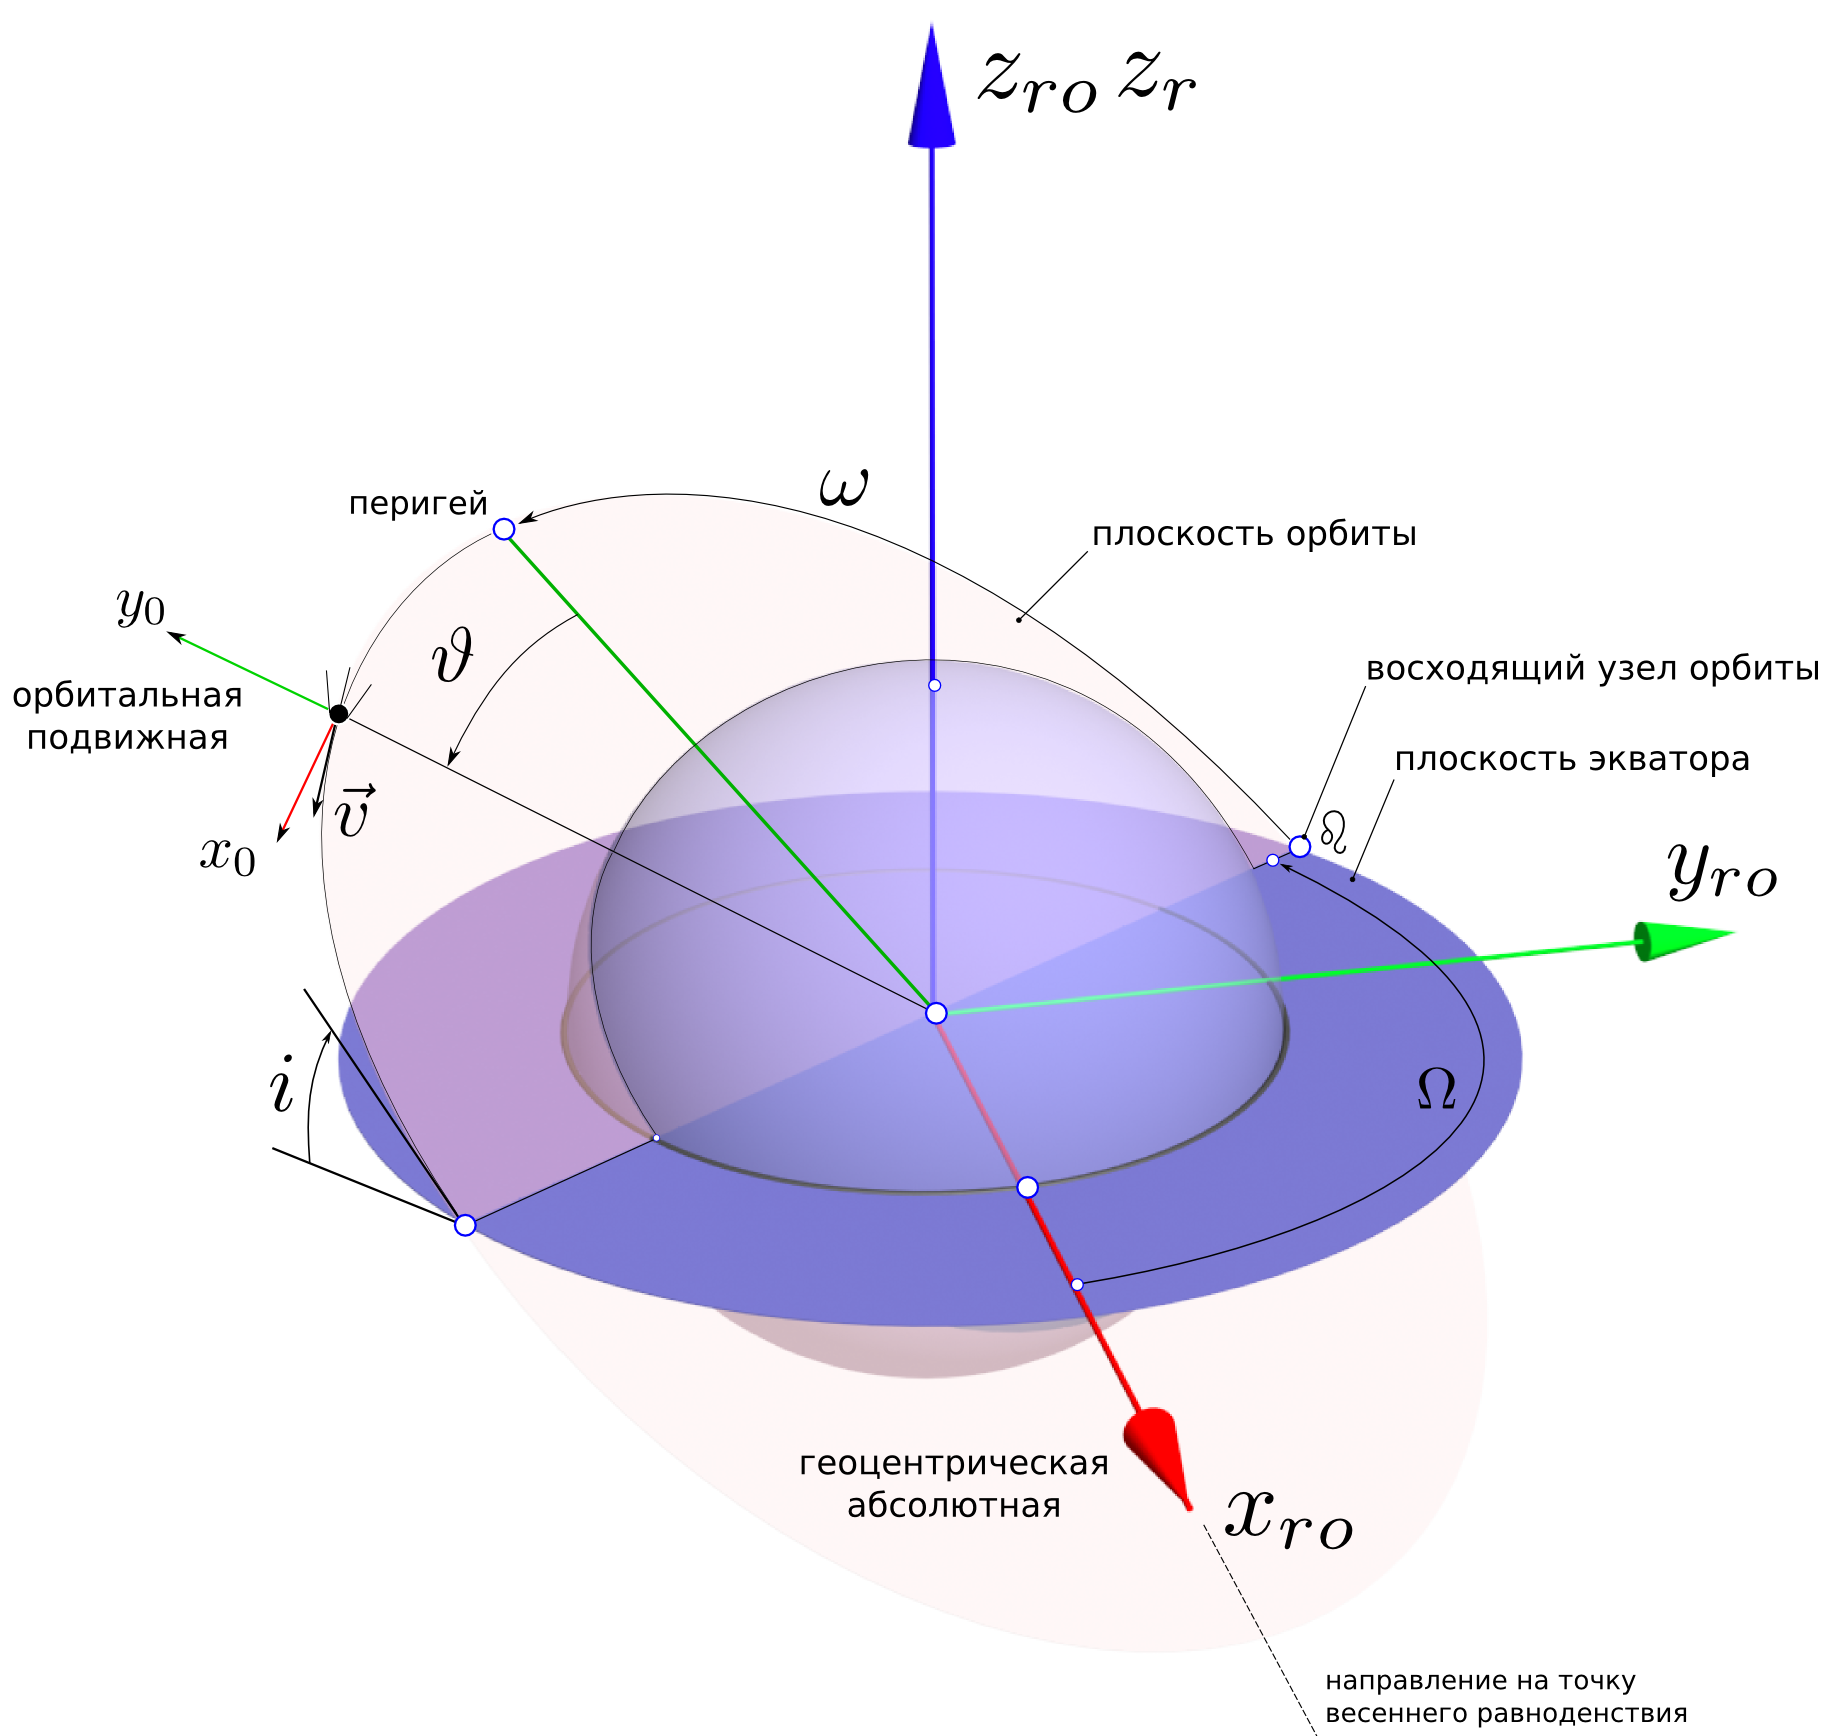
\includegraphics[width=1\textwidth]{orbit.png}
%\end{figure}
%\column{0.4\linewidth}
%\begin{itemize}
%  \item $a$ -- большая полуось,
%  \item $i$ -- наклонение,
%  \item $e$ -- эксцентриситет,
%  \item $\Omega$ -- долгота восходящего узла,
%  \item $\omega$ -- аргумент перицентра,
%  \item $\vartheta$ -- угол истинной аномалии,  
%\end{itemize}
%\end{columns}
%\end{frame}

\begin{frame}[fragile]{Приведение к ОДУ первого порядка}
$$
\left\{
\begin{aligned}
  & m a_x = F_x, \\
  & m a_y = F_y, \\
  & m a_z = F_z.
\end{aligned}\right. \quad \Rightarrow \quad
\left\{
\begin{aligned}
  & \dot v_x = F_x/m = - \mu \, x / r_0^3, \\
  & \dot v_y = F_y/m = - \mu \, y / r_0^3, \\
  & \dot v_z = F_z/m = - \mu \, z / r_0^3, \\
  & \dot x = v_x, \\
  & \dot y = v_y, \\
  & \dot z = v_z 
\end{aligned}
\right.
$$
Неизвестные функции: 
$$
  v_x, v_y, v_z, x, y, z
$$
\end{frame}

\begin{frame}[fragile]{Файл-функция правой части dqdt.m}
Вектор состояния:
$$
  q = (v_x, v_y, v_z, x, y, z)
$$
\begin{lstlisting}
function dq = dqdt(t, q) 
  global params;
  v = q(1:3);
  r = q(4:6);  
  % Вектор ускорения
  a = - params.mu*r/norm(r,2)^3;
  % Возвращаем производную вектора q
  dq = [a,v];
\end{lstlisting}
\end{frame}

\begin{frame}[fragile]{Главный файл-скрипт orbitalMotion.m}
\begin{lstlisting}
% Гравитационный параметр Земли
params.mu=3.986e14;
% Радиус Земли
params.Rz = 6371000;    
% Формируем вектор начальных условий  
% для круговой орбиты высотой
h  = 300000;
% Орбитальная скорость
V  = sqrt(params.mu/(params.Rz+h));  
q0 = [0;V;0;h+Rz;0;0];
% От 0 до одного орбитального периода
tk = 2*pi*(h+params.Rz)/V;
% Вызываем функцию интегрирования
[t,q] = ode45(@dqdt, q0, [0 tk]);  
\end{lstlisting}
\end{frame}

\begin{frame}[fragile]{Результат интегрирования}
Матрица $q$ содержит 6 столбцов и число строк равное числу шагов интегрирования, соотеветсвующие моментам времени, содержащимся в столбце $t$:
$$
  t = \begin{bmatrix} 0 \\ t_1 \\ t_2 \\ \ldots \\ t_n \end{bmatrix}, \quad
  q = 
\begin{bmatrix} 
  v_{x0} & v_{y0} & v_{z0} & x_{0} & y_{0} & z_{0} \\
  v_{x1} & v_{y1} & v_{z1} & x_{1} & y_{1} & z_{1} \\
  v_{x2} & v_{y2} & v_{z2} & x_{2} & y_{2} & z_{2} \\
  \ldots & \ldots & \ldots & \ldots & \ldots & \ldots \\
  v_{xn} & v_{yn} & v_{zn} & x_{n} & y_{n} & z_{n} 
\end{bmatrix}.
$$
\end{frame}

\begin{frame}[fragile]{Экспорт результатов в текстовый файл}
Для обработки результатов в других программах возможна запись таблицы с результатами в текстовый файл, в котором значения в каждой строке разделяются запятой:
\begin{lstlisting}  
  dlmwrite('results.csv',[t, q], ',');
\end{lstlisting}
$$
\begin{bmatrix} 
  t_0, & v_{x0}, & v_{y0}, & v_{z0}, & x_{0}, & y_{0}, & z_{0}, \\
  t_1, & v_{x1}, & v_{y1}, & v_{z1}, & x_{1}, & y_{1}, & z_{1}, \\
  t_2, & v_{x2}, & v_{y2}, & v_{z2}, & x_{2}, & y_{2}, & z_{2}, \\
  \ldots & \ldots & \ldots & \ldots & \ldots & \ldots & \ldots \\
  t_n, & v_{xn}, & v_{yn}, & v_{zn}, & x_{n}, & y_{n}, & z_{n} 
\end{bmatrix}.
$$
\end{frame}


\begin{frame}[fragile]{Построение графиков}
\matcode{Файл orbitalMotion.m}
\begin{lstlisting}
  plot(t, (sqrt(sum(q(4:6,:).^2,2))-Rz)*0.001);
  xlabel('t, c');
  ylabel('r, км');
\end{lstlisting}

\end{frame}

\section{Относительное орбитальное движение}

{
\usebackgroundtemplate{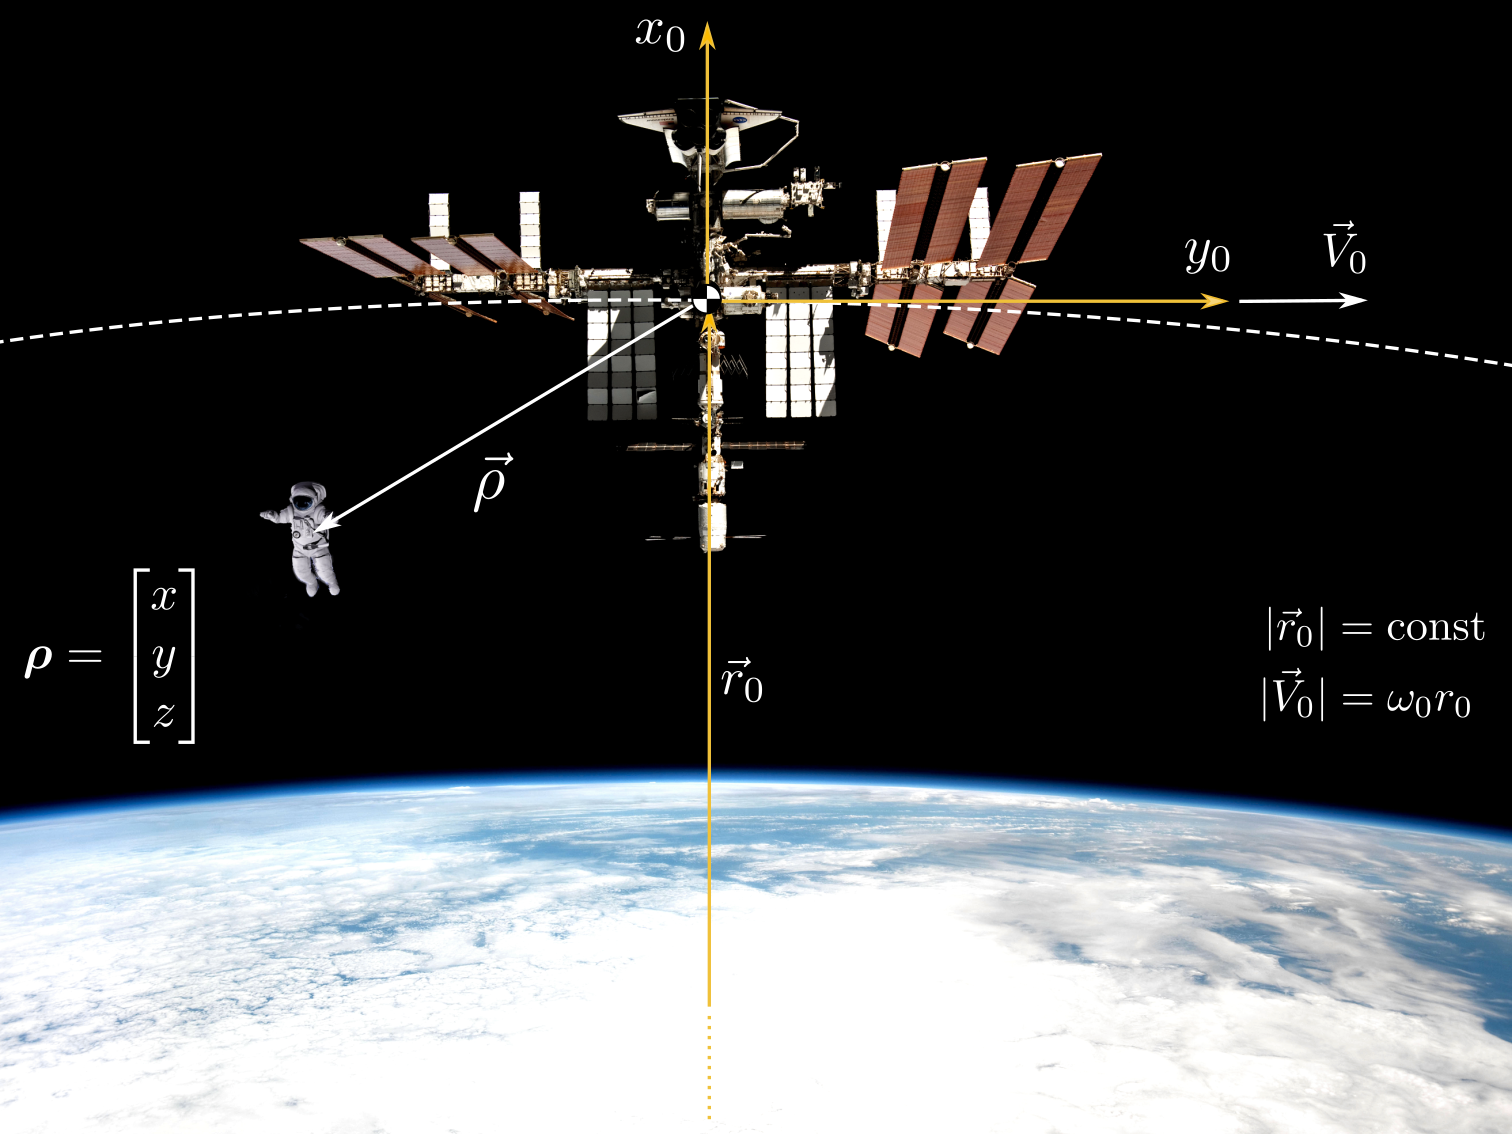
\includegraphics[width=\paperwidth,height=\paperheight]{./ManInSpace.png}}
\frame{}
}

\frame{
\frametitle{Направление осей системы координат $Ox_0y_0z_0$}
\begin{center}
 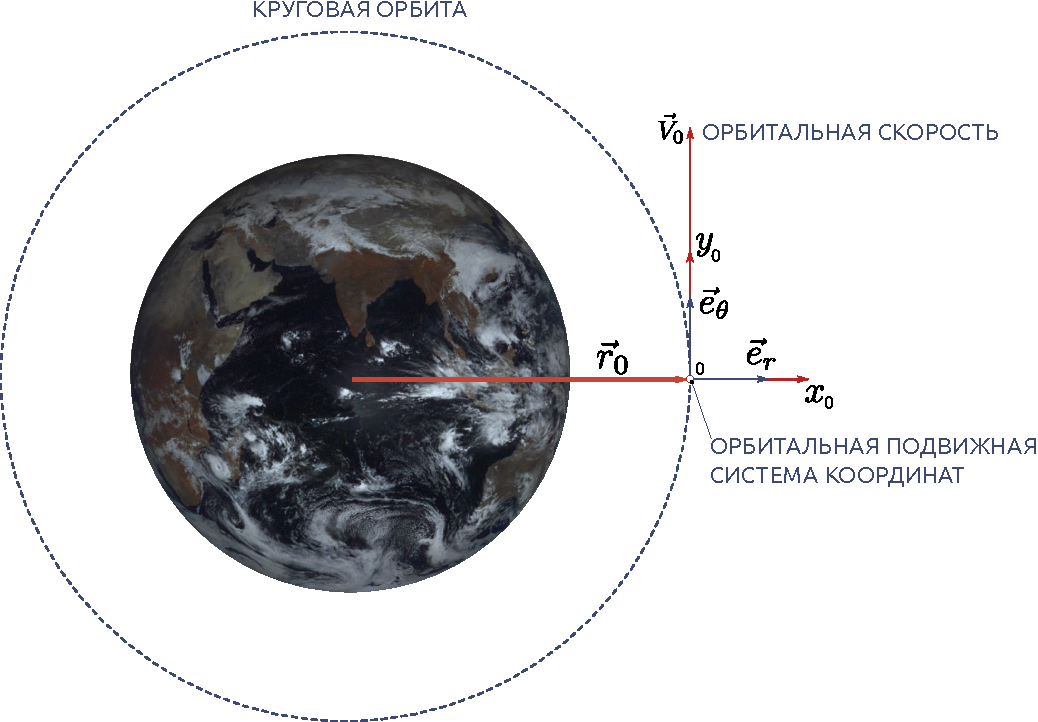
\includegraphics[width=1\linewidth]{./Orbital_SC.pdf}
\end{center}
}

\frame
{
\frametitle{Скорость движения по орбите}
Ускорение при движении по круговой орбите с постоянной скоростью
$$
  a_0 = V_0^{\;2}/r_0 = \omega_0^2 r_0
$$
Ускорение определяется силой притяжения:
$$ 
  a_0 = F / m = \mu / r_0^2 
$$
Скорость движения по круговой орбите:
$$
 \omega_0 = \sqrt{\frac{\mu}{r_o^3}}, \quad V_0 = \omega_0 r_0 = \sqrt{\frac{\mu}{r_0}}
$$ 
Период обращения по круговой орбите высотой $h_0$:
$$
 T = \frac{2 \pi}{\omega_0} = 2 \pi \sqrt{\frac{r_o^3}{\mu}} = 2 \pi \sqrt{\frac{(R_\Earth+h_0)^3}{\mu}}
$$ 
} 



\frame{
\frametitle{Движение орбитальной системы координат}
\begin{columns}
\column{0.4\linewidth}
\begin{figure}[htbp]
  \centering
  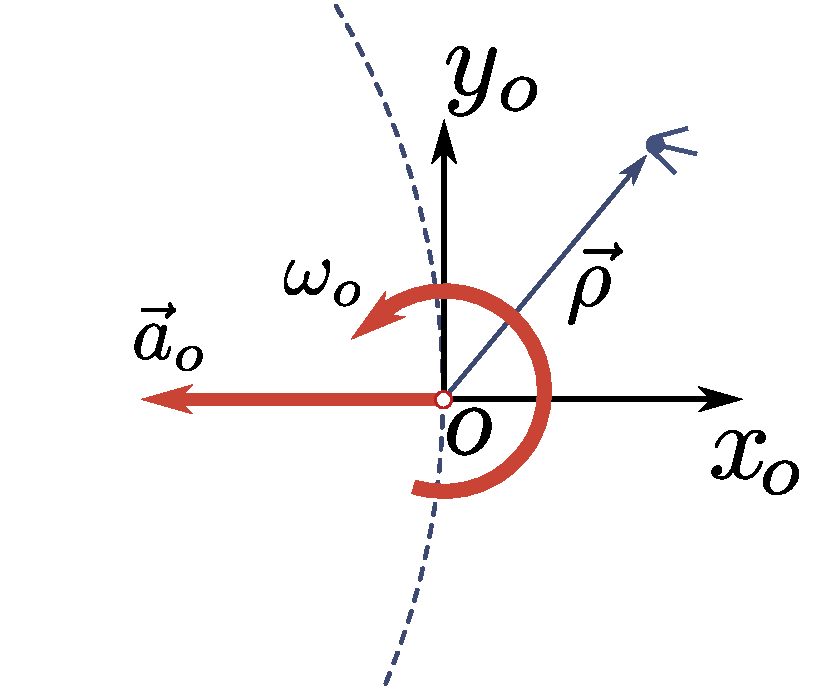
\includegraphics[width=0.95\textwidth]{non-inertial.pdf}
\end{figure}
\column{0.6\linewidth}
Система координат $Ox_0y_0z_0$ вращается с угловой скороcтью $\omega_o$  вокруг оси $Oz_o$
$$
  \boxed{\omega_o = \sqrt{\frac{\mu}{r_o^3}}}
$$
Начало системы координат  $Ox_0y_0z_0$  движется с ускорением
$$
\boxed{a_o=\omega_o^2 r_o=\frac{V_o^2}{r_o}}
$$
\end{columns}
}



\frame
{
\frametitle{Уравнения относительного движения КА}
\begin{columns}
\column{0.6\linewidth}
\begin{center}
 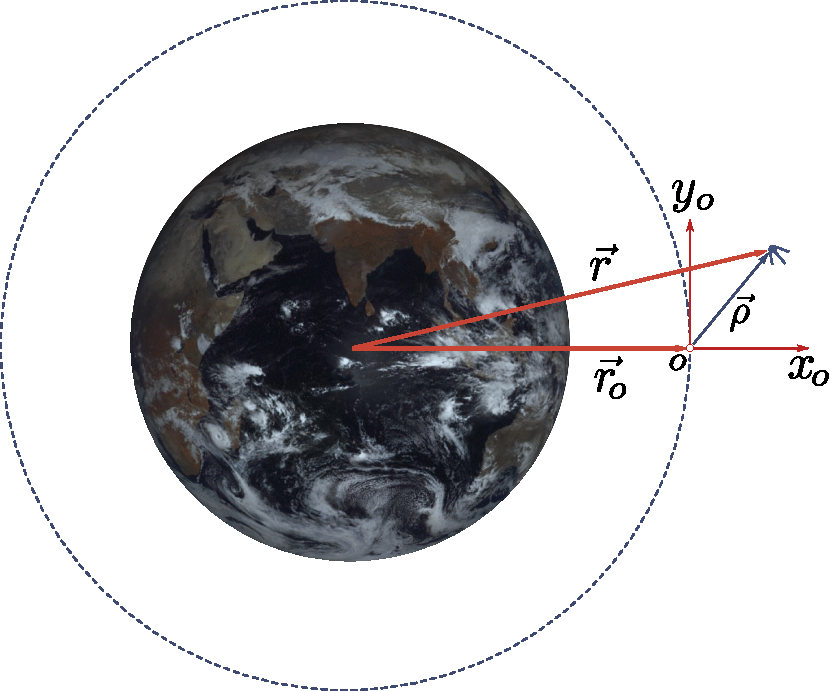
\includegraphics[width=1.0\linewidth]{./Orbital_SC_rho.pdf}
\end{center} 
\column{0.4\linewidth}
$$
  \boxed{m \ddot{\vec{\rho}} = \vec F + \vec F_e + \vec F_c}
$$
\begin{itemize}
 \item $\vec F_e$ -- переносная сила инерции
 \item $\vec F_c$ -- сила инерции Кориолиса
 \item $\vec F$ -- гравитационная сила
\end{itemize}
\end{columns}
}


\frame{
\frametitle{Дифференциальные уравнения относительного движения}
$$
  \boxed{m \ddot{\vec \rho} = \vec F + \vec F_e  + \vec F_c}
$$
\begin{itemize}
 \item $\vec F_e$ -- переносная сила инерции:
$$
  \vec F_e = - m \vec a_e = - m (\vec a_o + \vec \omega_o \times (\vec \omega_o \times \vec \rho))
$$
 \item $\vec F_c$ -- сила инерции Кориолиса:
$$
  \vec F_c = - m \vec a_c =  - 2 m \, \vec \omega_o \times \dot{\vec \rho}
$$
 \item $\vec F$ -- гравитационная сила.
\end{itemize}
}

\frame
{
\frametitle{Переносная сила инерции}
\begin{columns}
\column{0.4\linewidth}
\begin{center}
 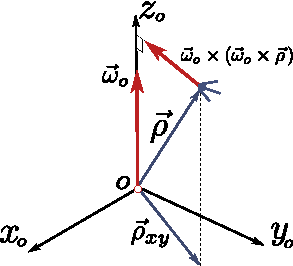
\includegraphics[width=1\linewidth]{./rho-rhop.pdf}
\end{center}
\column{0.6\linewidth}
$$
\vec F_e = - m \vec{a}_e = - m [\vec a_o + \vec{\omega}_o \times (\vec{\omega}_o \times {\vec \rho}\,)]
$$
\begin{align*}
  & \vec a_o = - \omega_o^2 \vec r_o \\
  & \vec{\omega}_o \times (\vec{\omega}_o \times {\vec \rho}) = - \omega_o^2 \vec \rho_{xy}
\end{align*}
$$
\boxed{\vec F_e = m (\omega_o^2 \vec r_o + \omega_o^2 \vec \rho_{xy})}
$$
\end{columns}
}


\frame{
\frametitle{Гравитационная сила}
$$
  \boxed{m \ddot{\vec \rho} = \alert{\vec F} + \vec F_e  + \vec F_c}
$$
Гравитационная сила, действующая на КА
$$
  \vec F = - G \frac{M_\Earth m}{|\vec r\,|^2} \cdot \frac{\vec r}{|\vec r\,|} = - \mu \frac{m}{|\vec r\,|^2} \cdot \frac{\vec r}{|\vec r \,|}
$$
\begin{equation*}
  \boxed{\vec F = - \mu \frac{m}{|\vec r\,|^2} \cdot \frac{\vec r}{|\vec r\,|} = - \mu \frac{m \, \vec r}{|\vec r\,|^3}}
\end{equation*}
}

\frame{
\frametitle{Уравнение движения}
После подстановки выражения, полученного для $\mu$ в выражение для гравитационной силы, действующий на КА 
$$
 \vec F = - \mu \frac{m \, \vec r}{|\vec r\,|^3}  = - \omega_o^2 \left(\frac{r_o}{r}\right)^3 m \vec r
$$
уравнение относительного движения КА принимает вид
\begin{equation}
  m \ddot{\vec \rho} = - \omega_o^2 \left(\frac{r_o}{r}\right)^3 m \vec r + m \, \omega_o^2 ( \vec r_o + \vec \rho_{xy})  - 2 m \, \vec \omega_o \times \dot{\vec \rho}
\end{equation}
или
\begin{equation}\label{eq:eq2}
  \boxed{\ddot{\vec \rho} = - \omega_o^2 \alert{\left(\frac{r_o}{r}\right)^3} (\vec r_o+\vec \rho \,) + \omega_o^2 ( \vec r_o + \vec \rho_{xy})  - 2 \, \vec \omega_o \times \dot{\vec \rho}}
\end{equation}
}

\frame{
\frametitle{Линеаризация $(r_o/r)^3$}
\begin{multline*}
  \left(\frac{r_o}{r}\right)^3 = \left(\frac{r}{r_o}\right)^{-3} = \left[\left(\frac{r}{r_o}\right)^2\right]^{-\frac{3}{2}} = \left[\frac{(\vec r_o+\vec \rho \, )^2}{r_o^2}\right]^{-\frac{3}{2}} = \\ =
  \left[\frac{r_o^2 + 2 \, \vec r_o \cdot \vec \rho + \rho^2}{r_o^2}\right]^{-\frac{3}{2}} = \left(\frac{r_o^2 + 2 \, r_o x + \rho^2}{r_o^2}\right)^{-\frac{3}{2}} = \\
  = \left(1+ \frac{2x}{r_o} + \textcolor{gray}{ \frac{\rho^2}{r_o^2} } \right)^{-\frac{3}{2}}
\end{multline*}
Т. к. $\rho \ll r_o$:
\begin{equation*}
 \boxed{\left(\frac{r_o}{r}\right)^3 \approx 1 - 3\frac{x}{r_o}}
\end{equation*}
}

\frame{
\frametitle{Линеаризованное уравнение движения}
\begin{multline*}
  \ddot{\vec \rho} = - \omega_o^2 \left(1 - 3\frac{x}{r_o}\right) \left(\vec r_o+\vec \rho \,\right) + \omega_o^2 ( \vec r_o + \vec \rho_{xy})  - 2 \, \vec \omega_o \times \dot{\vec \rho}_o
= \\ =
\underline{- \omega_o^2 \vec r_o} - \omega_o^2 \vec \rho + 3 \, \omega_o^2 \frac{x}{r_o} \vec r_o +  \textcolor{gray}{3 \, \omega_o^2 \frac{x}{r_o} \vec \rho} + \underline{\omega_o^2 \vec r_o} + \omega_o^2 \vec \rho_{xy} - 2 \, \vec \omega_o \times \dot{\vec \rho}_o
= \\ =
  3 \, \omega_o^2 \frac{x}{r_o} \vec r_o + \omega_o^2 (\vec \rho_{xy}-\vec \rho \,) - 2 \, \vec \omega_o \times \dot{\vec \rho}_o
\end{multline*}
}


\frame{
\frametitle{Линеаризованное уравнение относительного движения}
\begin{itemize}
 \item Векторное уравнение
$$
  \boxed{\ddot{\vec \rho} = 3 \, \omega_o^2 \frac{x}{r_o} \vec r_o + \omega_o^2 (\vec \rho_{xy}-\vec \rho \,) - 2 \, \vec \omega_o \times \dot{\vec \rho}}
$$
 \item Уравнение в координатной форме, в системе координата $Ox_oy_oz_o$
$$
  \begin{bmatrix} \ddot x \\ \ddot y \\ \ddot z \end{bmatrix} = 3 \, \omega_o^2 \frac{x}{r_o}
  \begin{bmatrix} r_o \\ 0 \\ 0 \end{bmatrix} +
  \omega_o^2 \begin{bmatrix} 0 \\ 0 \\ -z \end{bmatrix} -
  2 \begin{bmatrix} \vec i & \vec j & \vec k \\ 0 & 0 & \omega_o \\ \dot x & \dot y & \dot z \end{bmatrix}
$$
\end{itemize}
}

\frame{
\frametitle{Линеаризованные ДУ относительного движения}
Система дифференциальных уравнений:
$$
\left\{
\begin{array}{l}
  \ddot x = 3 \, \omega_o^2 x + 2 \omega_o \dot y, \\
  \ddot y = - 2 \, \omega_o \dot x, \\
  \ddot z = - \omega_o^2 z.
\end{array}
\right.
$$
Начальные условия:
$$
\begin{array}{l}
  x(0) = x_0, \;  y(0) = y_0, \; z(0) = z_0, \; \\
  \dot x(0) = \Delta V_{x}, \;  \dot y(0) = \Delta V_{y}, \; \dot z(0) = \Delta V_{z}.
\end{array}
$$
}

\begin{frame}[fragile]{Уравнения относительного движения}
Приближенные уравнения относительного движения*:
\begin{align*}
  & x = \frac{\Delta V_{x}}{\omega_0} \sin \omega_0 t - \frac{2 \Delta V_{y}}{\omega_0} \cos \omega_0 t + \frac{2 \Delta V_{y}}{\omega_0}., \\
  & y = 2 \, \frac{\Delta V_{x}}{\omega_0} \left( \cos \omega_0 t - 1 \right) + 4 \, \frac{\Delta V_{y}}{\omega_0} \sin \omega_0 t - 3 \, \Delta V_{y} t , \\
  & z =  \frac{\Delta V_{z}}{\omega_0} \sin \omega_0 t.
\end{align*}
Допущения:
\begin{itemize}
  \item орбита носителя круговая;
  \item расстояние между носителем и КА мало по сравнению с расстоянием от носителя до центра Земли;
\end{itemize}
{\scriptsize *Вывод уравнений приведён в \href{http://www.slideshare.net/tm_ssau/ss-17458335}{http://www.slideshare.net/tm\_ssau/ss-17458335}}
\end{frame}


\frame{
\frametitle{Отделение вдоль вектора орбитальной скорости}
\begin{columns}
\column{0.6\linewidth}
  \small $\Delta V_x=\Delta V_{z}=0, \Delta V_{y}=1$ м/с, $H=300$ км
\begin{center}
 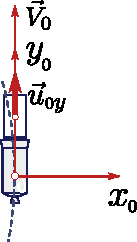
\includegraphics[width=0.3\linewidth]{./sepVy.pdf}
\end{center}
\begin{align*}
  & x(t) = \frac{2 \Delta V_{y}}{\omega_0} (1 - \cos \omega_0 t), \\
  & y(t) = 4 \, \frac{\Delta V_{y}}{\omega_0} \sin \omega_0 t - 3 \, \Delta V_{y} t , \\
  & z(t) = 0
\end{align*}
\column{0.4\linewidth}
\begin{center}
 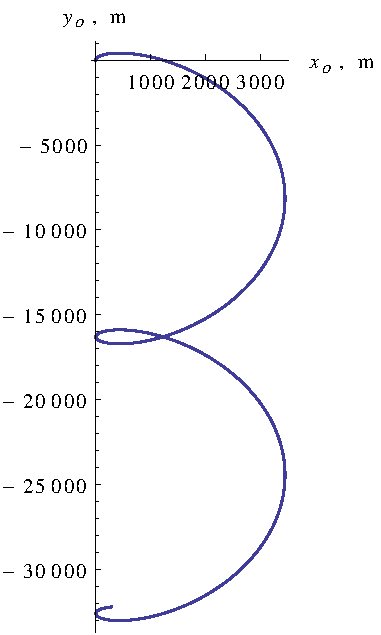
\includegraphics[width=1\linewidth]{./xyVy.pdf}
\end{center}
\end{columns}
}

{
\usebackgroundtemplate{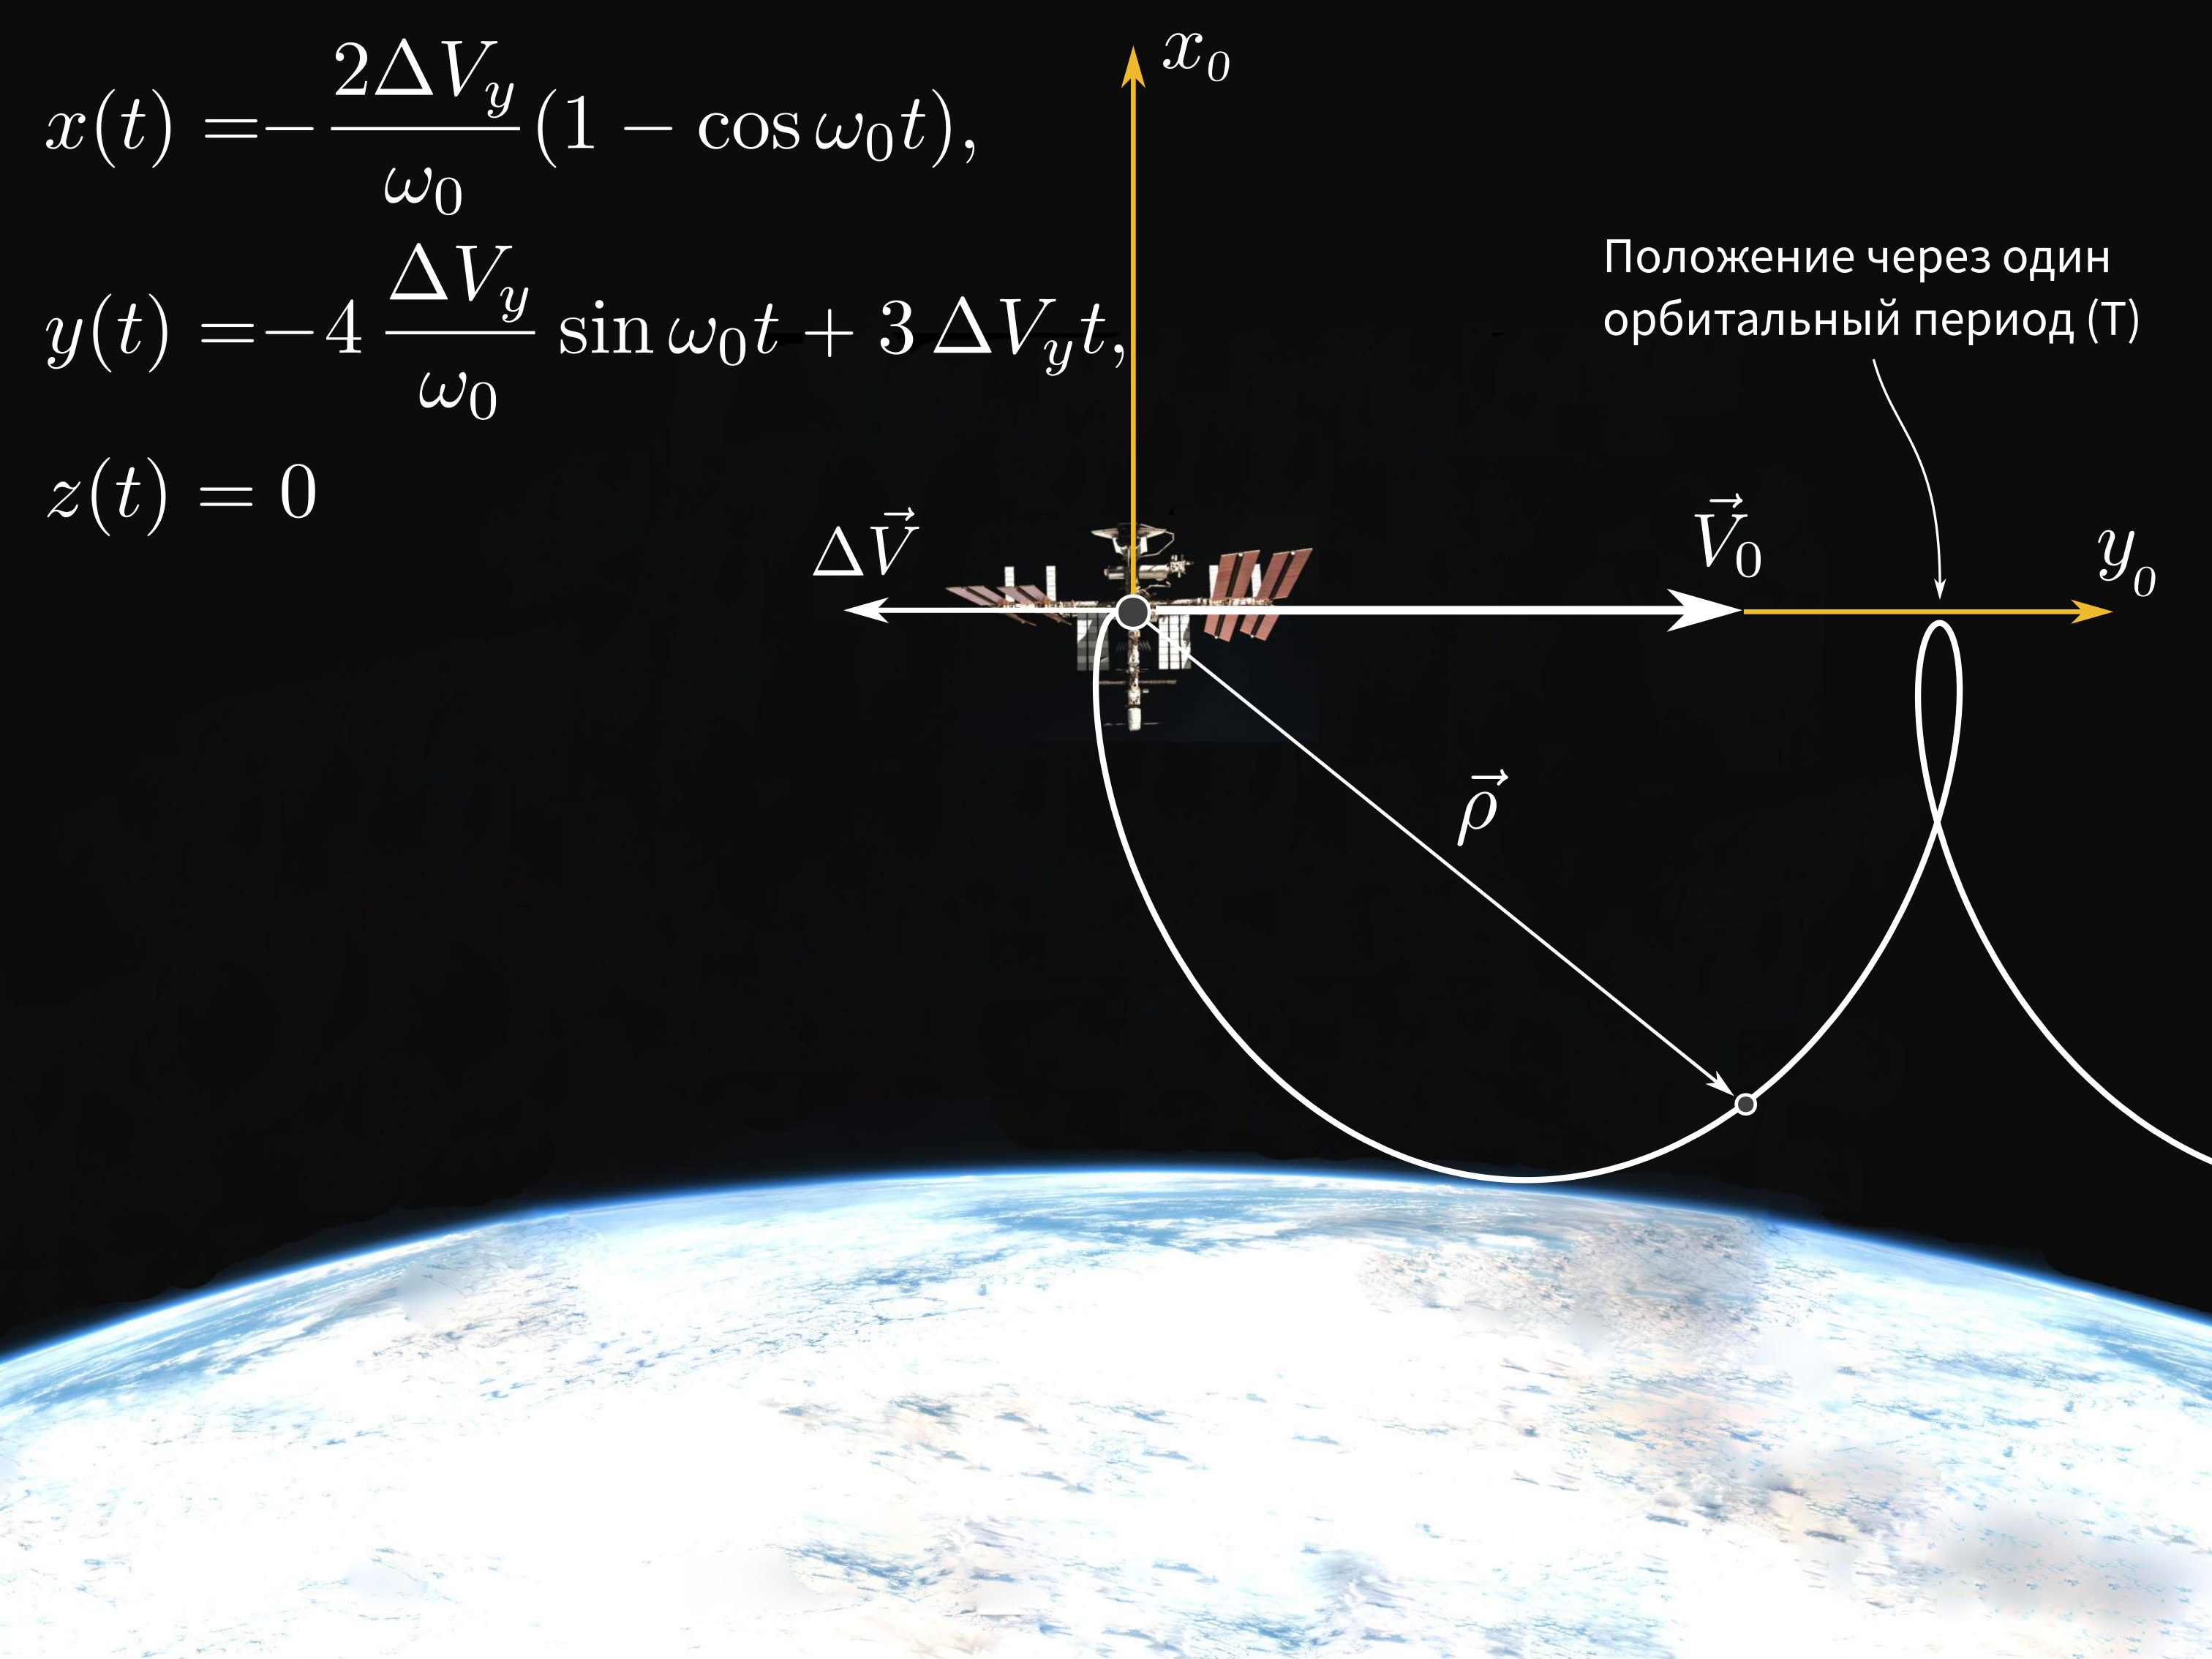
\includegraphics[width=\paperwidth,height=\paperheight]{./dV_back.png}}
\frame{}
}


{
\usebackgroundtemplate{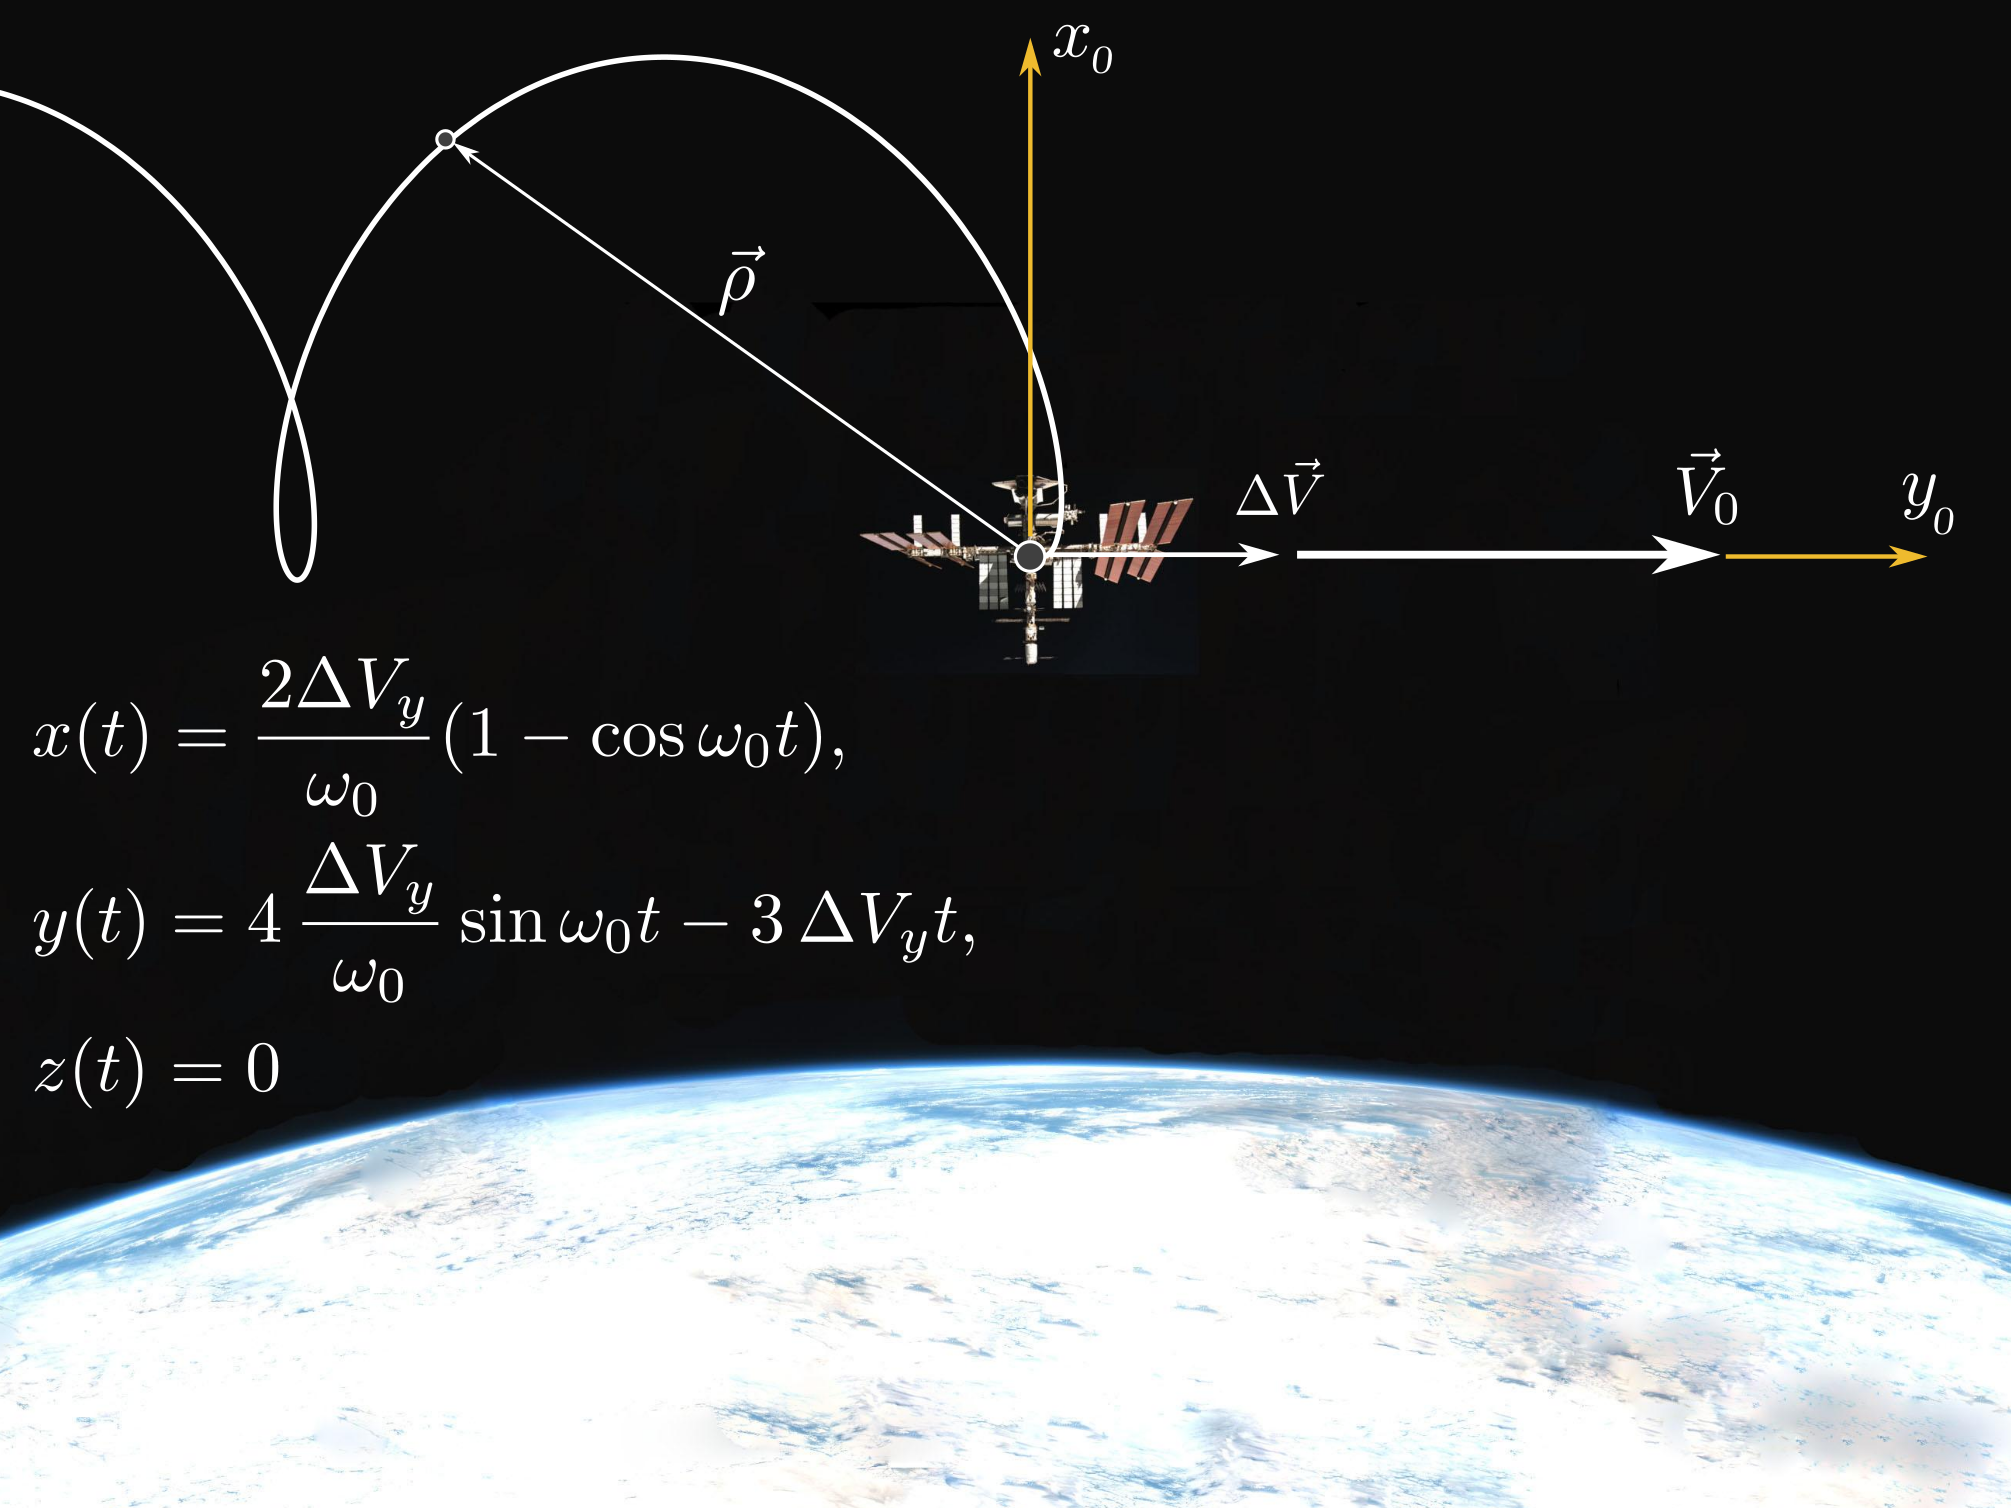
\includegraphics[width=\paperwidth,height=\paperheight]{./dV_forward.png}}
\frame{}
}

\frame{
\frametitle{Отделение вдоль радиус-вектора}
\begin{columns}
\column{0.6\linewidth}
$u_{0y}=u_{0z}=0$, $u_{0x}=1$ м/с, $H=300$ км
\begin{center}
 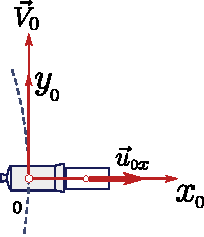
\includegraphics[width=0.45\linewidth]{./sepVx.pdf}
\end{center}
\begin{align*}
  & x(t) = \frac{\Delta V_{x}}{\omega_0} \sin \omega_0 t, \\
  & y(t) = 2 \frac{\Delta V_{x}}{\omega_0} \left( \cos \omega_0 t - 1 \right), \\
  & z(t) =  0
\end{align*}
\column{0.4\linewidth}
\begin{center}
 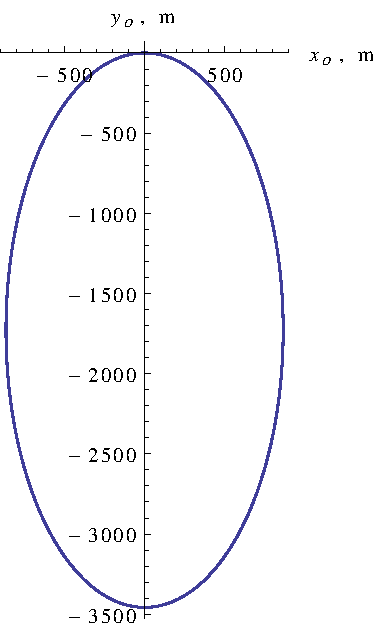
\includegraphics[width=1\linewidth]{./xyVx.pdf}
 % xyVx.pdf: 183x368 pixel, 72dpi, 6.46x12.98 cm, bb=0 0 183 368
\end{center}
\end{columns} 
}

{
\usebackgroundtemplate{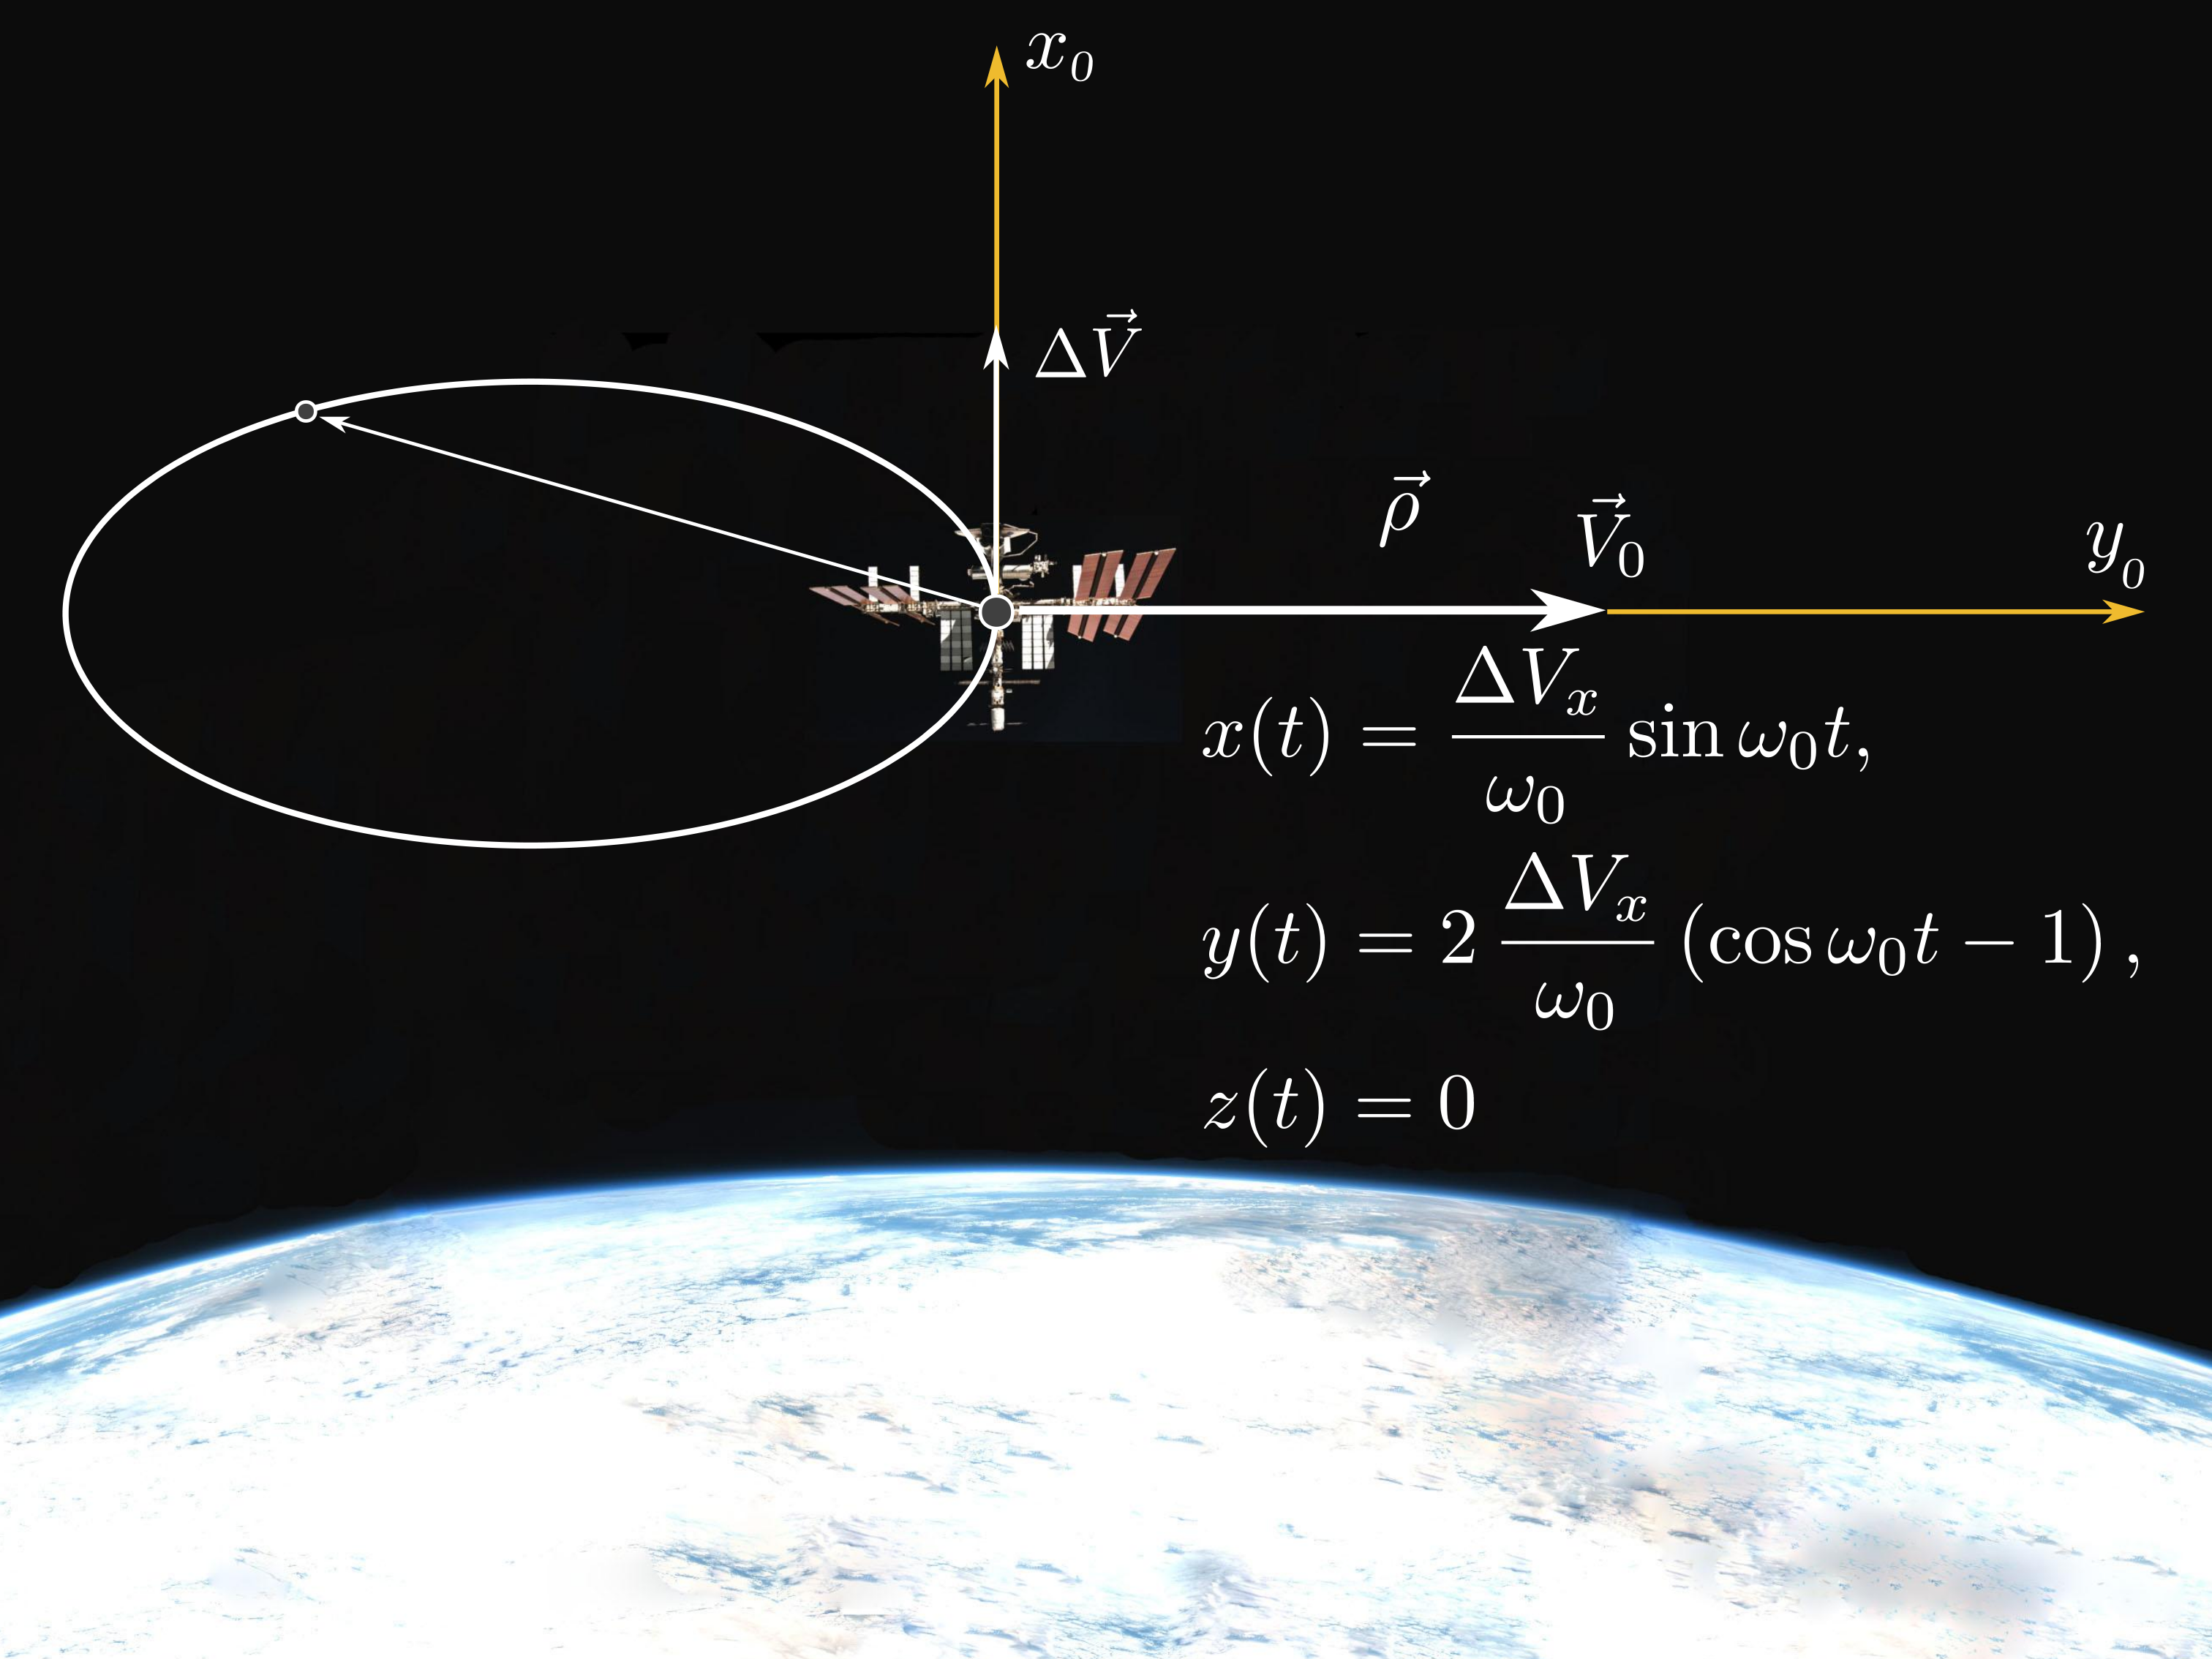
\includegraphics[width=\paperwidth,height=\paperheight]{./dV_up.png}}
\frame{}
}

\frame{
\frametitle{Отделение по нормали к орбите}
\begin{columns}
\column{0.45\linewidth}
\begin{figure}[htbp]
  \centering
  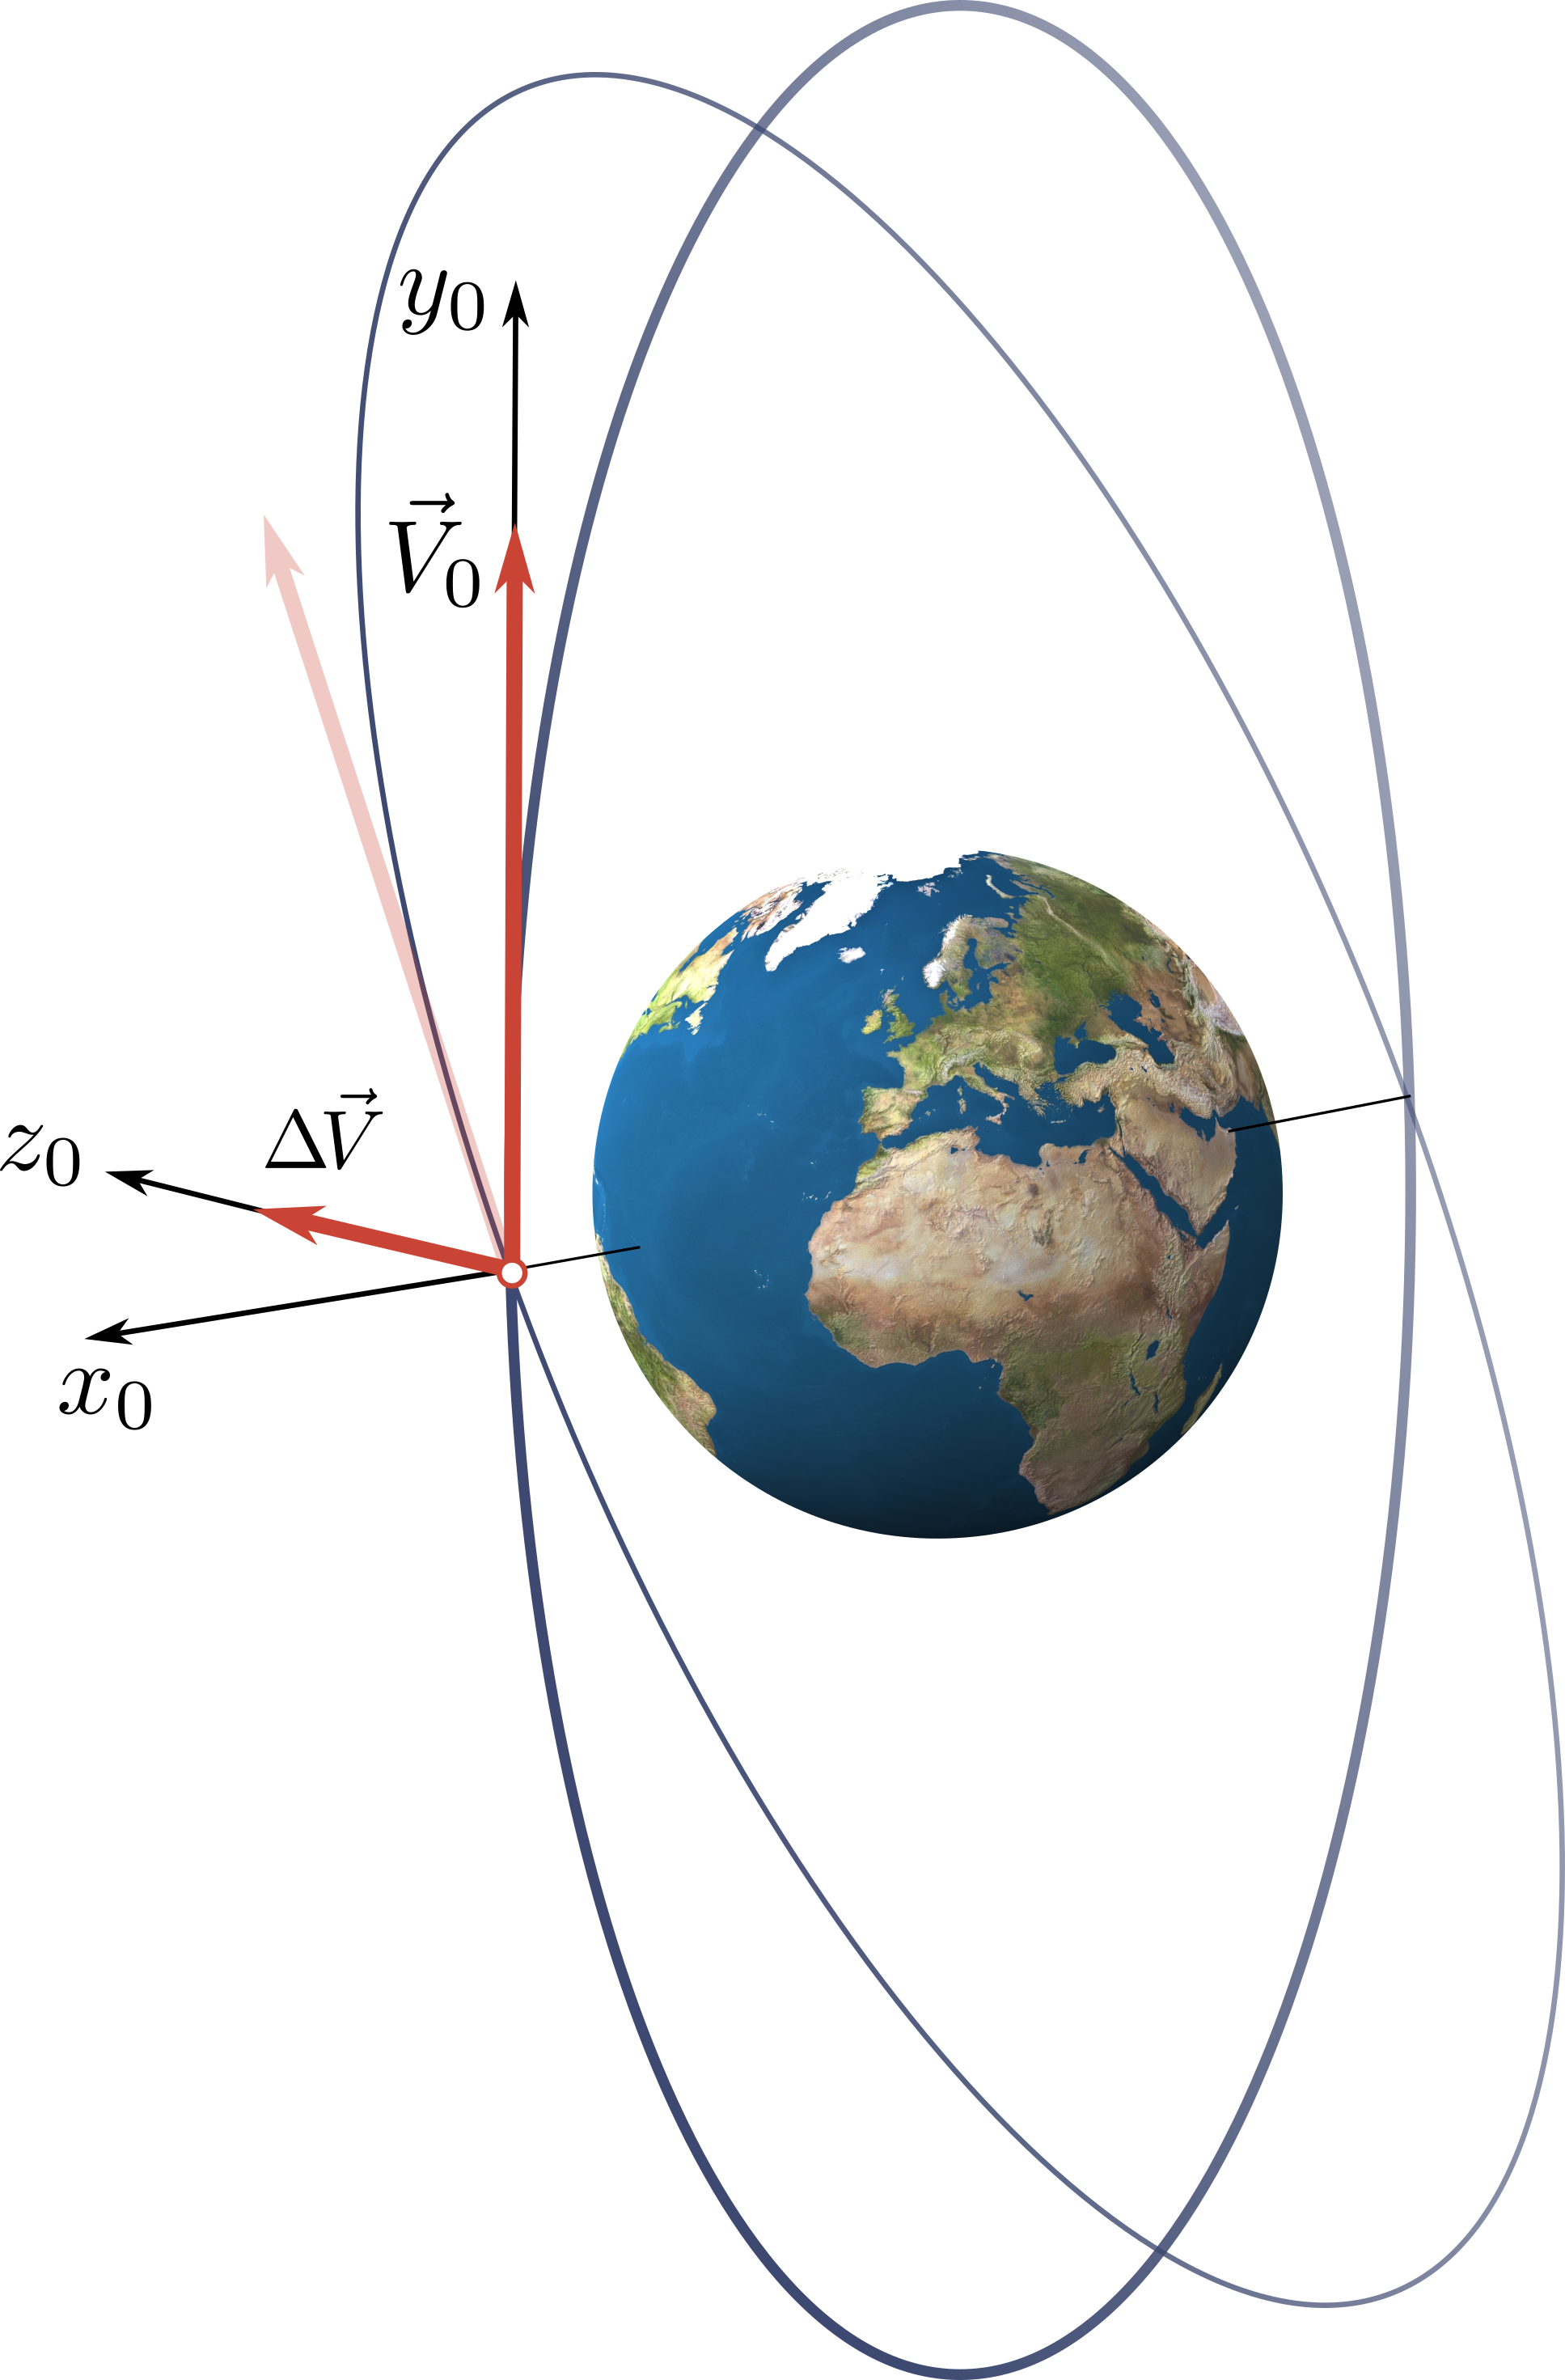
\includegraphics[width=1\textwidth]{dV_side.png}
\end{figure}
\column{0.55\linewidth}
$\Delta V_x=\Delta V_y=0, \Delta V_z=1$ м/с.
\begin{align*}
  & x(t) = 0, \\
  & y(t) = 0, \\
  & z(t) =  \frac{\Delta V_z}{\omega_0} \sin \omega_0 t
\end{align*}
\end{columns}
}

\frame{
\frametitle{Выводы}
\begin{itemize}
 \item При отделении КА вдоль нормали к плоскости орбиты происходит опасное сближение КА и носителя через половину орбитального периода.
 \item При отделении КА вдоль радиус-вектора носителя происходит опасное сближение КА и носителя через орбитальный период.
 \item Для безопасного отделения КА от носителя, вектор приращения скорости КА относительно носителя должен иметь проекцию на направление орбитальной скорости.
\end{itemize}
}

%
%
%
\section{Пересчёт координат из геоцентрической СК в орбитальную подвижную}
%
%
%
\begin{frame}[fragile]{Направления осей $Cx_oy_oz_o$}
\begin{columns} 
\column{0.5\linewidth} 
\begin{center}
 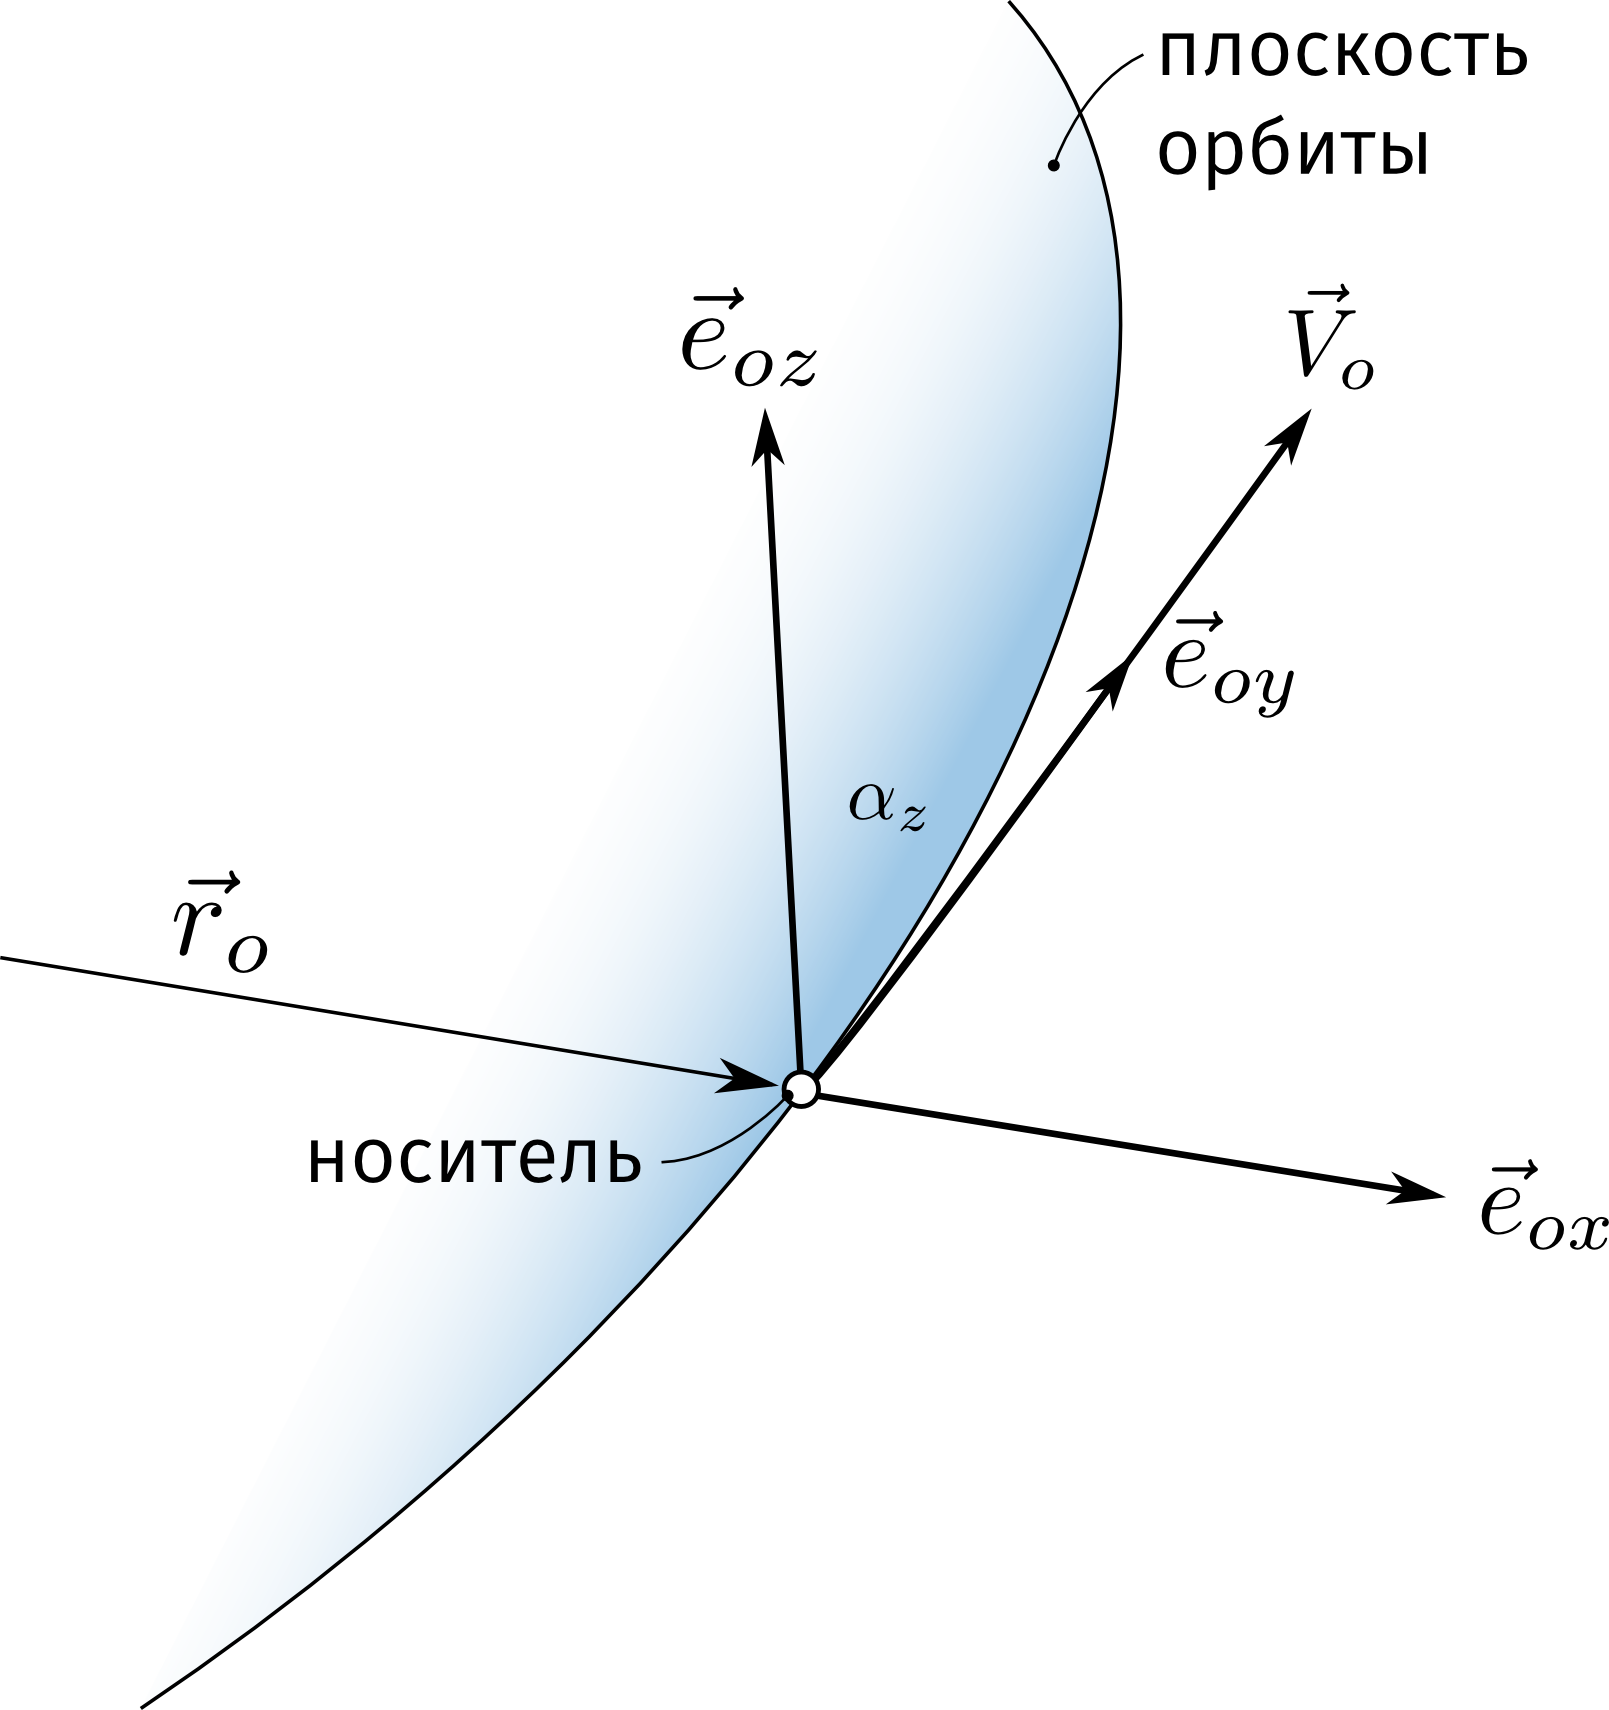
\includegraphics[width=1.1\linewidth]{./orbitalCoordinatesOnly.png} 
\end{center}
\column{0.5\linewidth} 
Единичный вектор радиус-вектора носителя:
$$
\vec e_{ox} = \vec r_0 / r_0.
$$
Единичный вектор нормали к орбите:
$$
\vec e_{oz} = (\vec r_0 \times \vec v_0) / | \vec r_0 \times \vec v_0 |.
$$
Единичный вектор трансверсали:
$$
\vec e_{oy} = (\vec e_{oz} \times \vec e_{ox})/| \vec e_{oz} \times \vec e_{ox} |.
$$
\end{columns}
\end{frame}


\begin{frame}[fragile]{Вектор относительного положения}
Матрица результатов интегрирования абсолютного движения двух материальных точек:
\begin{lstlisting}
q = 
v1x, v1y, v1z, x1, y1, z1, v2x, v2y, v2z, x2, y2, z2
v1x, v1y, v1z, x1, y1, z1, v2x, v2y, v2z, x2, y2, z2
...
\end{lstlisting}
Координатный столбец вектора положения второй точки относительно первой в проекциях на неподвижную систему координат:
\begin{lstlisting}
rho = q(:,10:12)-q(:,1:3);
\end{lstlisting}
\end{frame}

\begin{frame}[fragile]{Орты орбитальной подвижной системы}
\begin{lstlisting}
q = 
v1x, v1y, v1z, x1, y1, z1, v2x, v2y, v2z, x2, y2, z2
v1x, v1y, v1z, x1, y1, z1, v2x, v2y, v2z, x2, y2, z2
...
\end{lstlisting}
Координатные столбцы единичных векторов орбитальной подвижной системы координат, связанной с первым телом:
\begin{lstlisting}
r = sqrt( sum( q(:,4:6).*q(:,4:6) ,2) );
ex0 = q(:,4:6)./repmat(r,1,3);
\end{lstlisting}
\begin{lstlisting}[firstnumber=last]
v = sqrt( sum( q(:,1:3).*q(:,1:3) ,2) );
ev0 = q(:,4:6)./repmat(v,1,3);
\end{lstlisting}
\end{frame}

\begin{frame}[fragile]{Орты орбитальной подвижной системы}
\begin{lstlisting}
q = 
v1x, v1y, v1z, x1, y1, z1, v2x, v2y, v2z, x2, y2, z2
v1x, v1y, v1z, x1, y1, z1, v2x, v2y, v2z, x2, y2, z2
...
\end{lstlisting}
Единичный вектор нормали к плоскости орбиты:
\begin{lstlisting}
ez0 = cross(ex0,ev0,2);
ez0 = ez0./repmat(sqrt(sum(ez0.*ez0,2)),1,3);
\end{lstlisting}
Единичный вектор трансверсали:
\begin{lstlisting}[firstnumber=last]
ey0 = cross(ez0,er0,2);
ey0 = ey0./repmat(sqrt(sum(ey0.*ey0,2)),1,3);
\end{lstlisting}
\end{frame}

\begin{frame}[fragile]{Положение КА относительно носителя}
\begin{columns} 
\column{0.5\linewidth} 
\begin{center}
 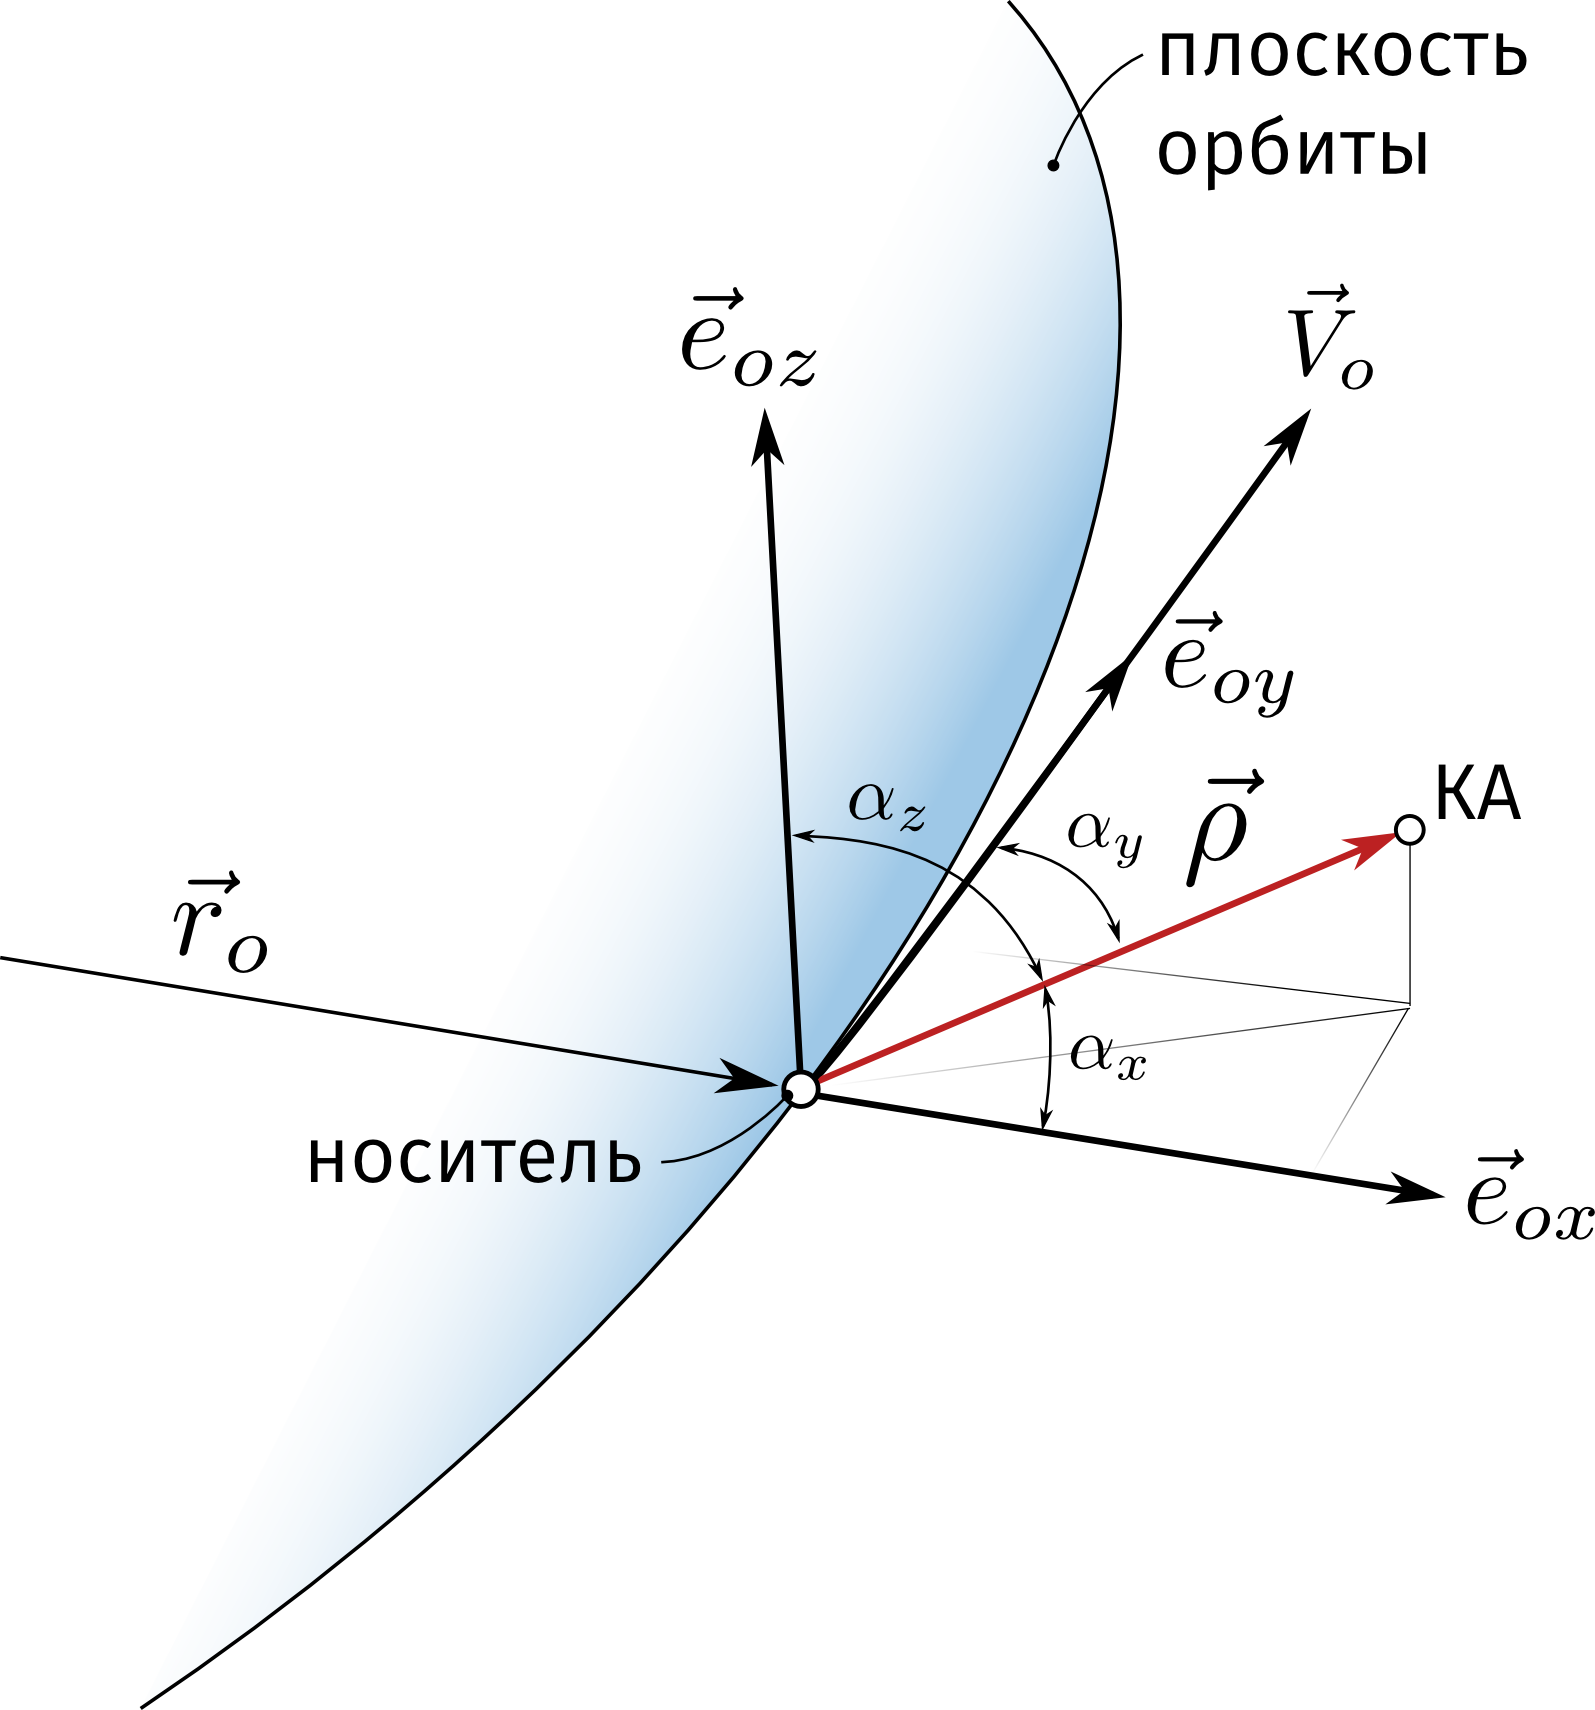
\includegraphics[width=1.1\linewidth]{./orbitalCoordinates.png} 
\end{center}
\column{0.5\linewidth} 
Радиус-вектор положения КА относительно носителя:
$$
\vec \rho = \vec r - \vec r_0
$$
Координаты КА относительно носителя в $Cx_oy_oz_o$:
$$
\begin{aligned}
  & x = \vec \rho \cdot \vec e_{ox}=\vec \rho \cos \alpha_x, \\
  & y = \vec \rho \cdot \vec e_{oy}=\vec \rho \cos \alpha_y, \\
  & z = \vec \rho \cdot \vec e_{oz}=\vec \rho \cos \alpha_z.
\end{aligned}
$$
\end{columns}
\end{frame}

\begin{frame}[fragile]{Относительное положение}
Координатный столбец вектора положения второй точки относительно первой в проекциях на неподвижную систему координат:
\begin{lstlisting}
rho = q(:,10:12)-q(:,1:3);
\end{lstlisting}
Тот же вектор в проекция на оси орбитальной подвижной системы:
\begin{lstlisting}
rho_o = [dot(rho,ex0,2),dot(rho,ey0,2),dot(rho,ez0,2)];
\end{lstlisting}
\end{frame}

\section{Задание}

\begin{frame}[fragile]{Групповое отделение КА}
  \begin{center}
    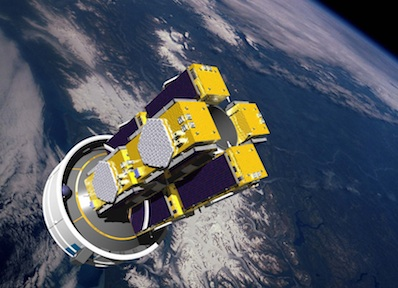
\includegraphics[width=0.8\linewidth]{ariane_galileo.jpg} 
  \end{center}
  \tiny{EADS Astrium}
\end{frame}

\begin{frame}[fragile]{Групповое отделение КА}
  \begin{center}
    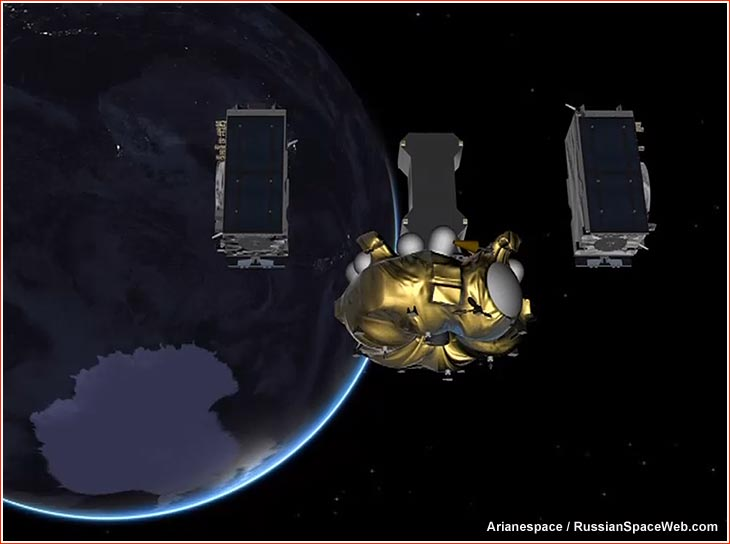
\includegraphics[width=0.8\linewidth]{sat_separation_1.jpg} 
  \end{center}  
\end{frame}


\begin{frame}[fragile]{Групповое отделение КА}
  \begin{center}
    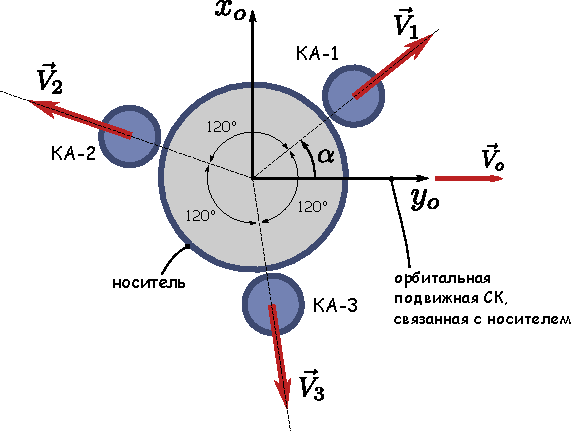
\includegraphics[width=0.9\linewidth]{./3KA.pdf} 
  \end{center}
\end{frame}


\begin{frame}[fragile]{Групповое отделение КА}
\begin{enumerate}
 \item[1.1] От носителя (орбитальной ступени) одновременно отделяется три малых космических аппарата. Векторы приращений скоростей малых КА относительно орбитальной ступени лежат в плоскости орбиты. Используя уравнения относительного орбитального движения, определите наилучший угол отделения КА. 
\end{enumerate} 
\end{frame}

\begin{frame}[fragile]{Групповое отделение КА}
\begin{enumerate} 
 \item[1.2] Постройте траектории движения КА относительно носителя (на одном рисунке).
 Постройте графики изменения расстояний между КА и носителем и между каждой парой КА (на одном рисунке).
 \item[1.3] Определите минимальное расстояние между КА и носителем и между каждой парой КА через один орбитальный период носителя. 
\end{enumerate} 
\end{frame}


\begin{frame}[fragile]{Групповое отделение КА}
\begin{enumerate} 
 \item[2.1] Напишите программу интегрирования дифференциальных уравнений абсолютного движения двух материальных точек (носитель и КА) в центральном поле. 
 \item[2.2] Сравните результаты, полученные в п. 1.2 (для одного из КА), с результатами полученными при интегрировании уравнений абсолютного движения двух материальных точек в центральном поле: найдите абсолютную погрешность определения положения КА относительно носителя в орбитальной подвижной системе координат, считая результаты интегрирования уравнений абсолютного движения точным решением.
\end{enumerate} 
\end{frame}


\plain{
\scriptsize 
Vadim Yudintsev\\
Computational Mechanics with MATLAB\\
Lecture 4: Orbital motion\\
\vspace{10pt}
LaTeX Beamer theme METROPOLIS\\
by Matthias Vogelgesang\\
\href{https://github.com/matze/mtheme}{https://github.com/matze/mtheme}
}
  
  
\end{document}
